    % TODO: Review Wang (2024) 
    
    \documentclass{article}
    \usepackage{longtable}
    % Language setting
    % Replace `english' with e.g. `spanish' to change the document language
    \usepackage[english]{babel}
    \setlength{\parindent}{0pt}
    \usepackage{parskip}
    
    % \usepackage{natbib}
    \usepackage[numbers]{natbib}
    \usepackage{tikz}
    \usetikzlibrary{arrows.meta,positioning,calc}
    \usepackage{subcaption}
    \bibliographystyle{abbrvnat}
    
    \usepackage{cancel}
    \usepackage{xcolor}
    \usepackage[normalem]{ulem}
    \newcommand{\DIFadd}[1]{{\color{blue}#1}}
    \newcommand{\DIFdel}[1]{{\color{red}\sout{#1}}}
    
    % Set page size and margins
    % Replace `letterpaper' with `a4paper' for UK/EU standard size
    \usepackage[letterpaper,top=2cm,bottom=2cm,left=3cm,right=3cm,marginparwidth=1.75cm]{geometry}
    
    % Useful packages
    \usepackage{amsmath}
    \usepackage{graphicx}
    \usepackage[colorlinks=true, allcolors=blue]{hyperref}
    
    \title{Advection impacts on water resources}
    \author{You}
    
    \begin{document}
    % \maketitle
    
    \begin{abstract}
    
    \end{abstract}
    
    
    
\section{Introduction}

% --- Opening: heterogeneity → advection → examples ---

The surface energy balance and the associated exchange of water vapor between the land surface and the atmosphere are routinely modelled under the assumption of horizontal homogeneity, yet most land surfaces are spatially heterogeneous.
Wherever surface properties change abruptly---at the boundary between an irrigated field and fallow land, at the shoreline of a lake, or at the margin of a snow-covered catchment---horizontal gradients in temperature and humidity drive the lateral transport of heat and moisture.
This process, referred to here as local advection, perturbs near-surface profiles of temperature and specific humidity and, in turn, modifies the turbulent fluxes of sensible and latent heat at the surface.
Its effects have been documented in a wide range of environments, including elevated evapotranspiration (ET) in irrigated fields bordered by dry land \citep{rao1974local}, enhanced evaporation from lakes and reservoirs \citep{higgins2013measured}, and accelerated snowmelt at exposed patch margins \citep{shook1997snowmelt, essery2006boundary}.

In some cases, sensible heat may be drawn from the overlying air to support evaporation, so that the latent heat flux exceeds the local net radiation---a phenomenon termed evaporative enhancement \citep{yang2013new, kool_within-field_2018}.
This occurs because warm, dry air moving over a cooler, well-watered surface provides an additional source of thermal energy that supplements net radiation \cite{spronken2000advection}.
While early analytical work often assumed a perfectly saturated surface \cite{lang1974influence, rao1974local}, more recent research has focused on how surface controls, such as stomatal resistance and surface relative humidity, shape energy partitioning within a soil--plant--atmosphere continuum \cite{baldocchi1995intra}.

% --- Why it matters: water resources ---

\paragraph{Advection and water resources.}
Quantifying advective enhancement is important for water-resources planning, particularly irrigation management in heterogeneous landscapes.
Near leading edges, where hot, dry air from adjacent fallow or barren areas increases evaporative demand over irrigated patches, lysimeter studies show that advection can raise ET on the order of 30--100\% above what local net radiation alone could support \cite{rijks1971water, rosenberg1978extreme, spronken2000advection}.
These effects cannot be neglected over mosaic irrigated--fallow land surfaces and are particularly consequential during early growth stages, when seedlings are most vulnerable to high temperatures and elevated vapor pressure deficits.

% --- Why it matters: remote sensing ---

\paragraph{Advection and remote sensing.}
Quantifying advection is also important for improving the accuracy of remote-sensing ET models.
Although remote sensing advances now enable routine ET mapping, most pixel-based approaches treat each pixel as vertically one-dimensional and therefore neglect horizontal transport of heat and moisture \cite{liou2014evapotranspiration, mcshane2017review}.
This limitation is especially problematic in advective settings, such as agricultural landscapes with patchworks of irrigated and fallow fields \cite{derardja2024advancements}.
A small number of recent studies incorporate advection explicitly into remote-sensing ET algorithms, including modifications to SEB \cite{liu2016regional} and SEBAL \cite{mkhwanazi2015sebal}, or use high-resolution thermal imagery to diagnose advective fluxes \cite{wang2024advection}; we discuss these in Section~\ref{sec:discussion}.
More broadly, advection poses an ongoing challenge for connecting high-resolution land-surface data with the coarse-resolution variables used in atmospheric models \cite{kustas_effects_2003}, because the magnitude of advective enhancement depends on background conditions, patch configuration, and stomatal feedbacks to the advected humidity deficit \cite{raupach_averaging_1982}.

% --- Land fallowing as a specific motivation ---

\paragraph{Land fallowing as a motivating application.}
In water-limited regions, land fallowing is increasingly used to reduce agricultural water consumption \cite{melton2014mapping}.
% TODO: fill in California numbers.
During the 2011--2015 California drought, for example, fallowed area in the Central Valley increased substantially as irrigated acreage was curtailed to conserve groundwater and surface-water supplies.
This trend raises a set of quantitative questions that current models are not well equipped to answer: How much water is actually saved by fallowing?  Are those savings partially offset by advective enhancement of ET on the remaining irrigated fields?  How sensitive is the net water balance to the spatial pattern of fallowed and cultivated parcels?

% --- Timeliness: RS advances ---

\paragraph{Timeliness.}
This topic is particularly timely, as advances in space-based satellites, aircraft, drones, and infrared cameras now provide the observational capability to resolve advective processes across scales---from individual field edges to regional mosaics \cite{volk2024assessing, fisher2020ecostress, derardja2024advancements}.
Yet remote sensing technologies remain under-leveraged in quantifying advection and its impacts on water resources \cite{liu2016regional}.
To exploit these new data streams, modeling frameworks must accommodate spatially variable boundary conditions derived from remote sensing.

% --- This study ---

\paragraph{This study.}
Here, we revisit Sutton's analytical solution for enhanced evaporation downwind of a dry--wet interface \cite{sutton1934wind} and develop an approach that bridges this classical framework with remote-sensing observations.
The application explored is specific to mosaic fallow and cultivated landscapes, where highly advective conditions have been repeatedly documented.

\begin{figure}
    \centering
    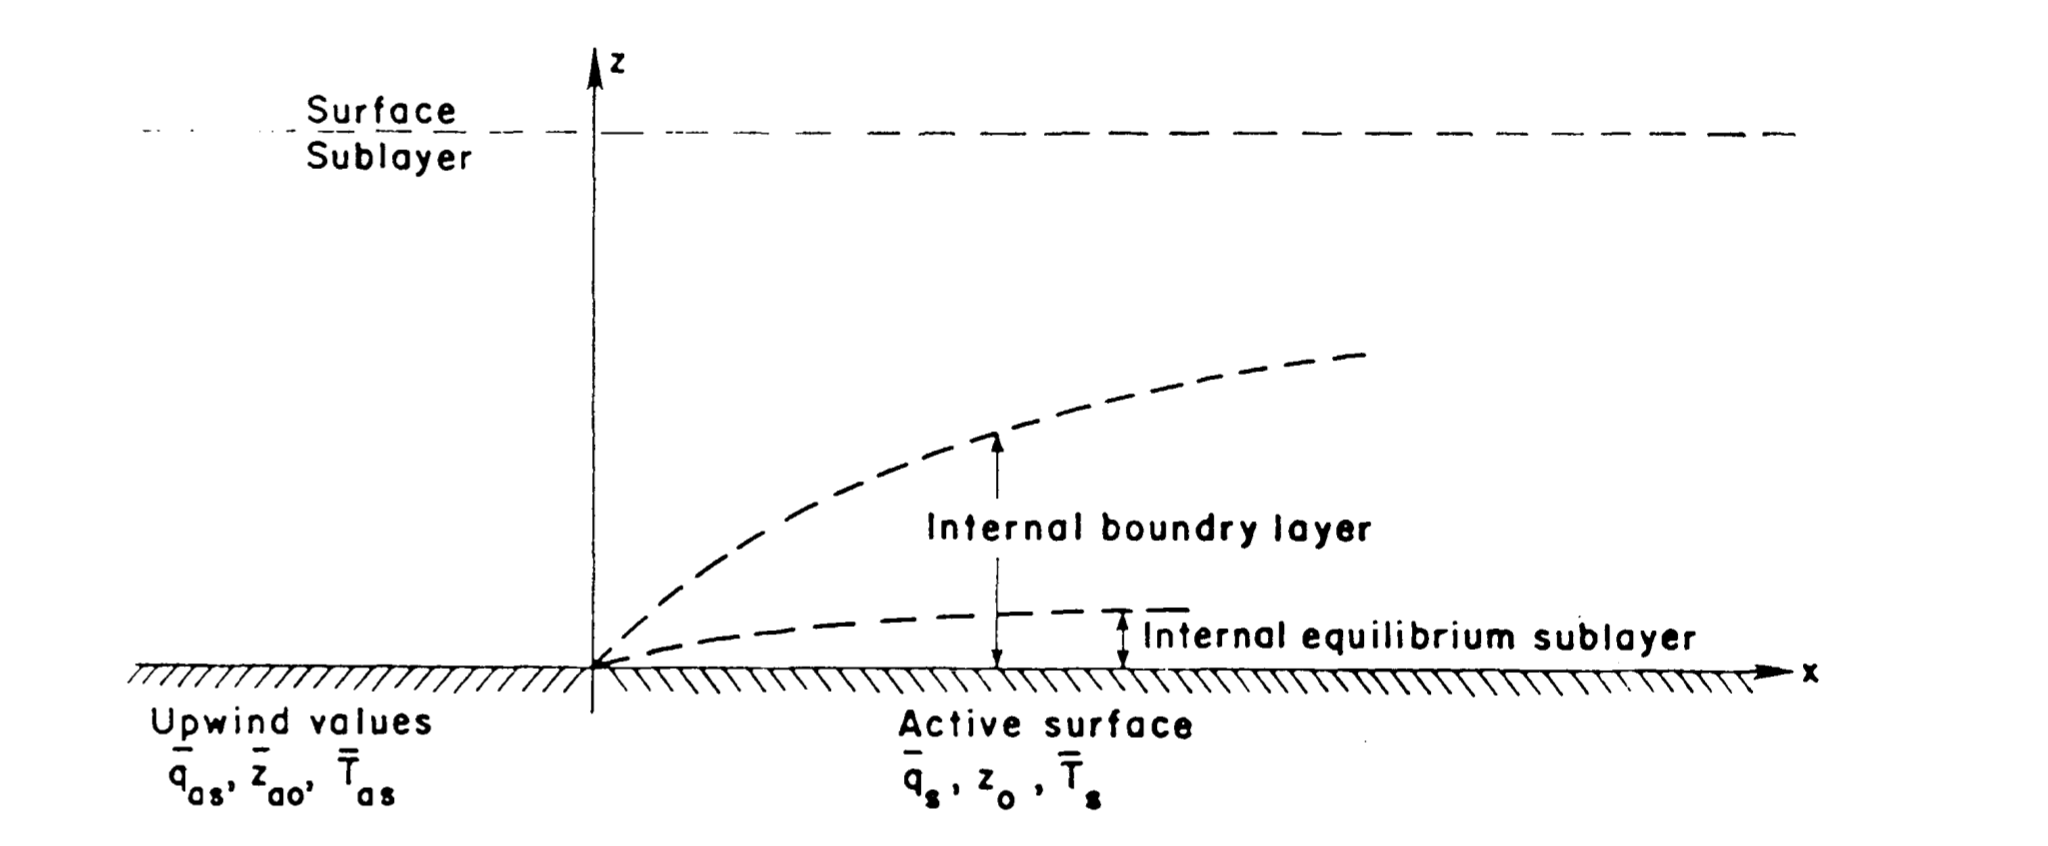
\includegraphics[width=0.8\linewidth]{figures/Figure7.1.png}
    \caption{Sutton's problem.  Definition sketch of the two-dimensional internal boundary layer that develops when air advects across a sharp transition in surface moisture, from an upwind dry, water-limited surface to a downwind wet or irrigated surface.  Upwind, strong sensible heating produces a warm, dry boundary layer; at the transition the surface switches abruptly to a wet, energy-limited regime.  An internal boundary layer grows with distance from the transition, within which temperature and humidity adjust toward values set by the wet-surface fluxes, while the overlying flow retains the properties of the upwind dry boundary layer.  \textit{Placeholder.}}
    \label{fig:7.1}
\end{figure}

\begin{figure}
    \centering
    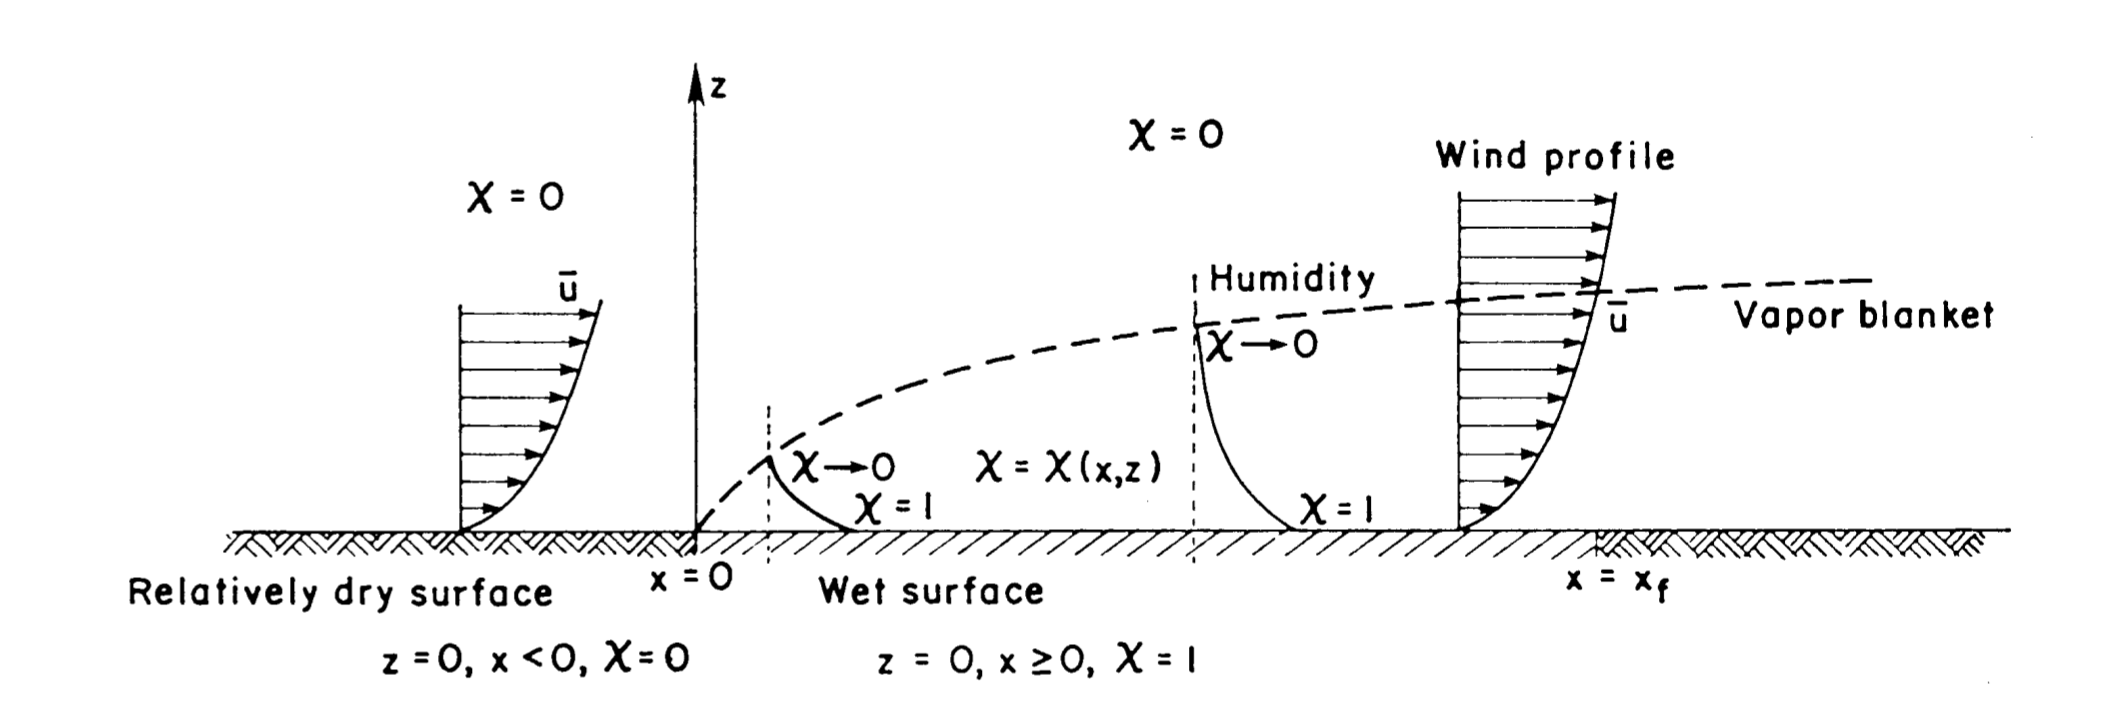
\includegraphics[width=0.8\linewidth]{figures/Figure7.3.png}
    \caption{Internal boundary layer of specific humidity in a dynamically uniform boundary layer.}
    \label{fig:placeholder}
\end{figure}

The paper is organized as follows.
Section~\ref{sec:review} reviews prior analytical, numerical, and observational work on advection.
Section~\ref{sec:methods} describes the governing equations, the first-order eddy-diffusivity closure, and the boundary-condition formulations used here; we show that this representation, although simpler than higher-order closures \cite{rao1974local}, yields plausible results for the contrasts of interest.
The results are presented in three parts:
(1)~comparison to the experimental observations of \citet{rider1963horizontal} and \citet{baldocchi_intra-field_1995}, demonstrating good agreement;
(2)~estimation of fallowing effects on ET relative to continuous cultivation; and
(3)~scenario exploration under warming atmospheric conditions.
Section~\ref{sec:discussion} discusses implications for water-resources management and remote-sensing ET models, and Section~\ref{sec:conclusion} summarizes the findings.
This work advances on previous studies by explicitly considering spatial configuration and wind direction in estimating advective enhancement.

\section{Review of prior work}
\label{sec:review}
    
    \subsection*{Early work} 

        Advection is a topic rich in tradition, addressed by various fields (micrometeorology, hydrology, agronomy, boundary-layer turbulence).

  \paragraph{Sutton's problem}
     
     
\citet{sutton1934wind} developed an analytical solution to the humidity transport equation for the case of a sudden change in surface conditions from a dry to wet surface.
% Brutsaert: The solution describes evaporation from a uniformly-moist surface of limited size, such as a lake or an irrigated field, whose temperature and roughness are uniform and the same as the surrounding presumably drier land surface. Under these simple conditions, the water vapor is a passive admixture that does not affect the dynamics of the motion or the stability. Hence, the problem can be considered non-dynamic and non-energetic and only the passive transfer of water vapor is of concern. This means that the wind profile fI = fI(z), v = w = 0, remains unchanged as the air travels past the humidity discontinuity
    
    \paragraph{Philip (1959)} 
    % 2) Philip (1959):
    % General “local advection” from horizontal heterogeneity: heat/moisture/momentum
    %  Two key mathematical moves
    % Similarity variable $\xi$ → PDE → ODE (incomplete gamma function solution)
    % Power-law $U(z)$ and $K(z)$ → tractable evaluation (tables; common exponents $m=1/7$, $n=6/7$)
    \citet{philip1959theory} expanded upon Sutton's 1934 work, developing an advection model describing the exchange of energy, moisture, or momentum due to horizontal heterogeneity.
    % providing the mathematical apparatus to solve for temperature and humidity diffusion fields in the lower atmosphere. 
    \citet{philip1959theory} advanced the mathematical tools to describe the advection problem by introducing a similarity variable  $\xi$, reducing the partial differential equations of vapor transport into a ordinary differential equation, and adopting power-law profiles for mean wind speed and eddy diffusivity (allowing evaluation via computational tables). 
    % Practical extensions beyond Sutton
    % Rough surfaces: applicability beyond aerodynamically smooth cases; extension Beyond Smooth Flow
    % Nonzero upwind moisture flux: introduce normalized scalar (e.g., $\chi$) / include $E_a$ for field relevance
    Whereas Sutton’s original solution was restricted to smooth flow, Philip’s approach accommodates aerodynamically rough    surfaces (which are more common in natural and agricultural lands). 
    %  Inclusion of Background Evapotranspiration
    Lastly, Sutton’s solution neglected evaporation from the dry land upwind of the wet area, and Philip's approach  included an upwind evapotranspiration rate, which made the model more broadly applicable.
    % Scaling outputs: clearer fetch dependence / internal boundary layer (vapor blanket) thickness; connection to mass-transfer formulas (via Brutsaert synthesis)
    % Better Scaling
     The updated solutions provided a clearer way to calculate the thickness of the `vapor blanket' (the internal boundary layer) as a function of the fetch (downwind distance). By using a power-law approximation for wind speed and eddy diffusivity, Philip provided a closed form that could be directly compared to observational results \cite{brutsaert2013evaporation}.
    
    Philip-type similarity solutions remain a common starting point for footprint-style advection corrections (cite), and continue to be used in applied agricultural micrometeorology (e.g., emission/advection-correction models such as FIDES; \cite{loubet2018fides}).
    
    Philip’s analytical approach relies on first-order closure, whereas later second-order closure models \citet[e.g., ][]{rao1974local} simulate turbulent covariances and can represent non-equilibrium adjustment, stability effects, and roughness changes across a discontinuity more mechanistically. 
    
     \paragraph{Energy balance constraints}
    
     % Early analytical work that combined specific humidity (q) and temperature (T) in advection, specifically adopting an energy balance perspective, moved beyond pioneering models like Sutton (1934), which treated water vapor as a passive scalar independent of the surface energy state
     Studies in the 1950s–1970s extended Sutton’s step-change framework by treating humidity $q$ and temperature $T$ as coupled through the surface energy balance, rather than as independent scalars with a fixed boundary condition. 
    Timofeev (1954), De Vries (1959), and Rider et al. (1963) examined the simultaneous local advection of moisture and heat, and how these variables affect the atmospheric stability and surface energy partitioning.
    Laikhtman (1964) presented an analytical solution in which surface temperature and humidity varies along the fetch under an energy constraint (from Brutsaert).
     \citet{yeh_solution_1971}  solved the coupled advection–diffusion system using Green’s functions, while tracking how  energy is partitioned downwind, including soil heat storage. 
    These models enforced local 1-dimensional energy balance of net radiation $R_n$ with sensible and latent heat fluxes,
    provided a mathematical description of 
    advective enhancement.
    
     % Townsend (1965): self-preservation as a complementary lens
    % Disturbance profiles become shape-invariant under appropriate scaling; dependence shifts to downstream distance $x$ (not initial details)
    \paragraph{Townsend (1965) -- self-preservation}
    \citet{townsend_response_1965,townsend_self-preserving_1965} introduced the assumption of self-preservation to the study of flow fields disturbed by abrupt changes in boundary condition.
    This approach assumes that the perturbation to the flow field caused by a change in boundary conditions is self-preserving, meaning that the disturbance profile remains shape-invariant under appropriate scaling: the flow's statistical properties, when scaled by local parameters, become independent of the initial conditions and depend only on the downstream distance $x$ as the thickness of the internal boundary layer increases \cite{antonia1977response}.
    
    %  A similarity approach about IBL growth/adjustment that can unify different step-change problems (heat/moisture/roughness)
    
    % Experimental support: Antonia et al. (1977)
    % Heated boundary-layer experiment framed explicitly as a self-preserving temperature disturbance beneath an external turbulent boundary layer
    
    Townsend's work has received support from laboratory experiments in \citet{antonia1977response}, who apply a self-preserving analysis to to their heated boundary-layer experiment of a temperature disturbance that grows underneath an external turbulent boundary layer. Their experimental results for the variation of thermal-layer thickness with fetch were in close agreement with the self-preserving results obtained by integrating Townsend's (1965) formulations.
      % TODO: add more detail for experiments and analysis
     
     % look for examples combining q and T using Sutton.
    
    \subsubsection*{1950s - 1970s: Impact of local advection on evaporation rates and plant water status}
    
    In the 1950s - 1970s, studies broadened in scope to consider controls other than micrometeorology, in particular, the role of stomates in controlling water losses  \cite{el1965effects, millar1964effect}.
    % agricultural studies documented advection impacts on ET using lysimeters to measure evapotranspiration and study the effects of advection on evaporation rates. 
    During this period, a series of agricultural studies documented significant advection impacts on ET utilized precision weighing lysimeters, particularly in arid and semi-arid environments \cite{rosenberg_extreme_1978}. 
    \citet{rosenberg1978extreme} documented record-breaking evapotranspiration rates in an irrigated alfalfa field during a severe drought in the midwestern United States: on clear mid-summer days, net radiation could support at most $\sim$7~mm/d of ET, yet sensible heat advection increased evapotranspiration to 10--14~mm/d.
    Allen et al.\ (2011) observed similar magnitudes in an irrigated agricultural area surrounded by desert, where lysimeter measurements recorded actual evapotranspiration rates that significantly exceeded the energy supplied by local net radiation, with ratios of ET/$R_n$ exceeding 2 in some instances --- demonstrating that dry air from the surrounding desert provides the additional thermal energy required to drive these extreme evaporation rates.
        
    % 1.  shift in the literature
    % Early “atmospheric demand → ET increases” assumption
    % Later recognition: vegetation is a regulated surface (stomatal control)
    % 2. Example Millar (1964): local advection linked to evaporation rate + plant water status (physiology enters the story)
    % 3. Mechanism: negative feedback under advection
    % Hot/dry air → higher VPD → stomatal closure can reduce/limit $LE$ (Baldocchi and Rao, 1995)
    %  Energy-partition consequence (observable signature)
    % 4. Closing stomata increases resistance → shifts energy from $LE$ toward $H$ → warmer surface (“thermostat”/partitioning effect) (Wang et al., 2024)
    % Takeaway for modeling
    % 5. Crops ≠ free-water surfaces; advection impacts depend on physiology + micrometeorology, not micrometeorology alone
    
     
    \subsection*{1970s onwards: Higher-order closure}
    
    
     Sutton’s (1934) approach, and other early models, had significant  limitations. Specifically, they (i) generally neglected the effects of roughness change at surface transitions, (ii) ignored thermal stratification (buoyancy effects), treating moisture as a passive scalar, and (iii) relied on assumed power-law forms for wind speed and eddy diffusivity that did not adapt to non-equilibrium conditions.
     
     The 1970s saw the application of higher-order closure models to address the advection problem, which addressed these limitations. 
     
     % Rao developed a second order closure scheme, which  addressed these limitations in Sutton's approach  including the effects of thermal stratification and surface roughness.
    
      \citet{rao1974local} developed a second-order turbulence closure model to simulate flow from a smooth dry surface to a grassy wet surface. The model includes equations for the mean quantities, turbulent fluxes, and the viscous dissipation rate, and solves a system of coupled partial differential equations for the mean wind speed, temperature, and humidity in the internal boundary layer.
      
    The Rao et al. (1974) model addressed limitations in Sutton's (1934) work by incorporating surface roughness and stratification (the model explicitly accounts for buoyancy  and roughness changes), and predicting the mean wind, temperature, and humidity fields such that both energy and moisture balances at the surface are satisfied.
    \citet{rao1974local} `showed that higher-order closure methods can become a powerful tool in the numerical analysis of evaporation problems with local advection (Brutsaert). 
    
    Subsequent field studies, such as \citet{baldocchi_intra-field_1995} continued to use predictions from this 1974 model as the baseline for comparison against direct eddy-covariance measurements of momentum, heat, and moisture.
    
    % Other studies to track down... 
     Donaldson (1973) and Mellor (1973) ...  
    
    \subsection*{1980s onward:  Footprint analyses}
    
    In the late 1980s and early 1990s, footprint analyses, in which the flow field is specified but scalar fields vary, also became a major focus of research.
    Schmid and Oke (1988)...
    \citet{schuepp1990footprint} presents one of the first widely used analytical models integrated into eddy-covariance software, offering a more rigorous approach to the 100:1 rule.
    
     % Lagrangian stochastic models, specified Flow Fields: Flow field is specified but scalar fields vary
    These models require the Eulerian velocity field (the wind profile) to be specified a priori to drive the model and predict the resulting particle trajectories of scalars like water vapor or heat \cite{hsieh_lagrangian_1997}.
    
    % TODO: details. 
    Specific releases were used to test these theories...  
    In particular, testing flow field done with point releases.
    Leclerc et al. (1988) used circular line sources to simulate tracer concentration fields inside plant canopies. 
    
    \subsection*{1990s onward}
    
     While research in the 1980s often relied on footprint analyses,  where the flow field was specified and scalar fields varied, the 1990s marked a shift toward understanding  feedback mechanisms between  the atmosphere and  biosphere.
     Soil, plant, and atmosphere was increasingly recognized as an integrated continuum, with atmospheric conditions and biological responses directly regulating one another.
     Models from this period 
     % moved beyond treating scalars as passive, 
     explored how atmospheric humidity deficits influence stomatal conductance, and how this alters the energy available for sensible and latent heat \cite{baldocchi1995intra}.
     
     
      % TODO follow up on these:  (Kroon and deBruin, 1993; McAneney et al., 1994; Brunet et al., 1994).
    
    
    \citet{baldocchi_intra-field_1995} found that the advection of hot dry air did not enhance surface evaporation rates near the upwind edge of the potato field, because of negative feedbacks among stomatal conductance, humidity-deficits, and evapotranspiration.
    % used a soil-plant-atmosphere model to examine feedbacks between humidity, stomatal conductance and evaporation, interpreting data with this model. 
    Thus, the advection of dry air over actively transpiring vegetation may not necessarily increase evaporation if negative feedback causes stomatal closure \cite{philip1987advection, baldocchi1995intra}. 
       
    \subsubsection*{Numerical advances}
    
     In the 1990s, the coupling of the flow field and scalar variables also gained attention.
     
    Researchers  increasingly used advances in simulation approaches -- such as large-eddy simulation (LES) or direct numerical solution (DNS) of the Navier–Stokes equations -- to investigate turbulent flow over surfaces with different roughness statistics, secondary circulations and energy balance closure.
    LES  emerged as a  tool for upscaling because it can dynamically simulate how surface heterogeneity impacts the atmospheric boundary layer \cite{albertson2001large}.
    
    Also in this period, \cite{albertson2001large} combined  remote sensing  with LES to study the interaction between heterogeneous land surfaces and the atmospheric boundary layer. 
    \citet{kustas2003effects} combined LES and remote sensing data, allowing for for detailed representation of soil and vegetation contributions to mass and energy exchanges.
    
     LES studies to follow up on: 2010s and 2020s (e.g., Eder et al., 2015; Kenny et al., 2017; Zhou et al., 2023).
    
    \subsection{Late 1990s onward: field experiments and advances in  measurement}
    
    \textbf{Measurements of turbulence during advection. }
    
    % Studies that explicitly measure turbulence structure and advective terms with multi-tower or profile setups.
    The 1990s saw advances in measuring turbulence structure and advective terms with multi-tower and multi-level systems 
    in agricultural lands \cite{baldocchi_intra-field_1995} , 
    forests \cite{staebler2004observing}, 
    mountains \cite{hammerle2007eddy, yi2008contribution}, and 
    coastal transitions \citep{allen2007satellite, rey-sanchez_evaporation_2017}.
    These advances were enabled by the 
    maturation and widespread adoption of reliable fast-response 3-D sonic anemometry and gas analyzers,
    increasing standardization of eddy-covariance methods \cite{fisher_ecostress_2020},
    and improved data logging and storage.
    In addition to these technical advances, coordinated field programs and networks provided the funding and coordination for  large flux-network field campaigns (e.g., AmeriFlux, EuroFlux, FLUXNET, and related campaigns).
    
    % Experiments over forests and complex terrain show that horizontal and vertical advection can be comparable in magnitude to the turbulent flux, particularly at night under stable stratification and in sloping terrain. 
    
    \subsection{Late 1990s onward: Advection in other fields }
    
    During this period, advection began to receive attention beyond boundary-layer meteorology, including in studies of ice, snow, and soil–atmosphere interactions.
    \textit{This period was marked by increasing attention to advection in other fields, including ice, snow, and soil interactions. }
    For example, Sutton's solution  was  adapted by  \citet{higgins2013measured} to examine water vapor advection near a lake–land transition using lidar data, showing good agreement between Sutton's solution and data.   
    
    \paragraph{Advection of sensible heat from bare soil to snow patches.}
    Patch-scale boundary-layer models in \citet{shook_snowmelt_1997} and \citet{essery_boundarylayer_2006} show that advective sensible heat can boost melt over patch edges.
    
    % To model advection to snow patches, Weisman (1977) applied mixing length theory, implicitly accounting for both latent heat advection (LEA) and sensible heat advection (HA).  `An obstacle to the development of an energy balance model for calculating melt quantities is the lack of reliable methods for evaluating the sensible heat flux. A priority research need is the development of “bulk methodologies” for calculating this term, especially for patchy, snow-cover conditions.' Gray et al. (1986)
    
    \citet{harder_simple_2019}
    
    
    % TODO: connects to advection impacts on soil moisture?
    
     % Carbon community – advection played a major role in C fluxes from ecosystem.
    The problem of underestimated night-time CO$_2$ fluxes in forest ecosystems led to advances in measurement of advective fluxes.
    
     Field campaigns in forests showed that nighttime CO$_2$ advection and storage can be similar in magnitude to the eddy flux, and can substantially alter annual NEE if included \cite{aubinet2003horizontal, marcolla2005importance, yi2008contribution, feigenwinter2008comparison, etzold2010contribution}. 
    % control-volume Eucalyptus experiment (Leuning 2008) 
    
    % ADVEX experiments and follow-ups indicate that including advective terms changes the latent-heat budget more than the sensible-heat budget, and improves energy-balance closure only partially, indicating the difficulty of quantifying advective impacts on $LE$ \cite{moderow2009available, moderow2021energy}.
    
    \subsection{Remote sensing: energy balance closure and role of advection}
    
    A full accounting of remote sensing for problems listed in introductions still awaits.
    
    Remote sensing observations are highly derived quantities. Observe at multiple scales. Remote sensing ecosystem stresses. 
    
    % Remote sensing: similar developments.
    On the remote sensing side, in parallel, the remote sensing as it pertains to this problem has experienced its own growth. 
    Nonlocal warming observed in deforestation studies \cite{cohn_forest_2019}.
    
    \subsection{Advection in remote-sensing ET models}
    
    Modifications to RS-based ET models such at SEBAL and SEB have relied on 
    (a) calibration to tower data and assumptions about closure, 
    (b) parametizations of warming potential of the atmosphere.
    
    
    
    These advances have demonstrated improvement in prediction; however, these models do not consider spatial configuration.
    In fragmented or patchy landscapes, under arid conditions, patches talk to each other. 
    
    Remains to bridge Sutton to remote sensing. 
    
    Horizontal advection contributes to surface-energy-balance non-closure: the full control-volume budget includes storage and advective flux-divergence terms, so a residual in $R_n - G - (H+LE)$ can reflect transport in addition to measurement errors. 
    
    

This study revisits Sutton's classical framework for advective enhancement of evapotranspiration across surface discontinuities and develops an approach to connect it with remote sensing observations. Section 2 reviews the evolution of advection theory, from Sutton's (1934) analytical solution and Philip's (1959) generalizations through higher-order closure models, footprint analyses, and recent large-eddy simulation studies, and summarizes how remote sensing ET models have addressed — or neglected — horizontal transport. Section 3 presents the governing equations for coupled heat and moisture advection under first-order eddy-diffusivity closure, describes the numerical solution procedure, and formulates three sets of boundary conditions: one for comparison against field experiments, one driven by satellite-derived land surface temperature, and one for scenario exploration under changing atmospheric conditions. Section 4 evaluates the model against the experimental observations of Rider et al. (1963) and Baldocchi and Rao (1995), then applies it to estimate how land fallowing patterns and warming temperatures affect advective enhancement of ET in irrigated–fallow mosaics. Section 5 discusses implications for water resources management, the potential to integrate the advection framework into operational remote sensing ET products such as OpenET, and the limitations and extensions of the approach. By explicitly accounting for spatial configuration and wind direction — factors absent from current pixel-based ET models — this work offers a pathway toward physics-based representation of advection in remote sensing evapotranspiration estimation.
    
    
    \section{Methods}
    
    The analysis/simple model follows approach outlined in \citet{brutsaert2013evaporation}, and implemented by \citet{higgins2013measured}.   
    We first describe for the simple case of a single dry patch upwind of a wet/irrigated patch, then how to generalize/adapt to mosaic/2-dimensional lands.
    In this case, input to model are equilibrium boundary conditions far-afield either size of the transition. 
    
    \subsection{Conservation equations}  
    
    \begin{table}
    \renewcommand{\arraystretch}{1.3} 
    \caption{Variables and constants}
    % \small
    \centering
    \begin{tabular}{lp{6cm}cl}
    \hline
    \textbf{Symbol} & \textbf{Definition} & \textbf{Equation/Value} & \textbf{Units} \\
    \hline
    & Variables &  & \\
    \hline
    $q$ & Absolute humidity &  &  g m$^{-3}$ \\
    $RH$ & Relative humidity &  &  g m$^{-3}$ \\
    $T$ & Temperature &  &  $C$ \\
    $LE$ & Latent heat flux & $L_v \overline{w'q'}$ & W/m$^2$  \\
    $H$ & Sensible heat flux & $\rho_{air} c_p \overline{w'T'}$ & W/m$^2$ \\
    $R_n$ & Net radiation &   & W/m$^2$ \\
    $G$ & Ground heat flux &   & W/m$^2$ \\
    $\bar{u}, \bar{v}, \bar{w}$ & Wind &   & m/s \\
    $z_{om}$ & Momentum roughness length &  & m \\
    $z_{max}$& Blending height / top of domain &  & m \\
    \hline
    & Constants &  & \\
    \hline
    $L_v$ & Latent heat of vaporization & $2.5 \cdot 10^6$ & J/kg \\
    $\rho_{air}$ & Density of air & $1.225$ & kg/m$^3$ \\
    $c_p$ & Specific heat of air at constant pressure & $1005$ & J/(kg K) \\
    $k$ & von Karman constant   & 0.4 &  \\
    \hline
    \end{tabular}
    \end{table}
    
    \begin{table}[t]
    \renewcommand{\arraystretch}{1.35} 
    \caption{Variables, parameters and constants}
    \centering
    \begin{tabular}{l p{6.0cm} p{5.2cm} l}
    \hline
    \textbf{Symbol} & \textbf{Definition} & \textbf{Equation/Value} & \textbf{Units} \\
    \hline
    \multicolumn{4}{l}{\textit{Variables}}\\
    \hline
    $q$ & Absolute humidity &
    $q=\dfrac{e}{R_v\,T}$ &
    kg m$^{-3}$ \\
    $RH$ & Relative humidity &
    $RH=100\,\dfrac{e}{e_{\mathrm{sat}}(T)}$ &
    \% \\
    $T$ & Air temperature &
    $T[\mathrm{K}]=T[^\circ\mathrm{C}]+273.15$ &
    K \\
    $\overline{w'q'}$ & Turbulent vertical flux of water vapor (mass) &
    $\overline{w'q'}=-K_q\,\dfrac{\partial \bar q}{\partial z}$ &
    kg m$^{-2}$ s$^{-1}$ \\
    $\overline{w'T'}$ & Turbulent vertical heat flux (kinematic) &
    $\overline{w'T'}=-K_t\,\dfrac{\partial \bar T}{\partial z}$ &
    K m s$^{-1}$ \\
    $LE$ & Latent heat flux &
    $LE=L_v\,\overline{w'q'}$ &
    W m$^{-2}$ \\
    $H$ & Sensible heat flux &
    $H=\rho_{\mathrm{air}} c_p\,\overline{w'T'}$ &
    W m$^{-2}$ \\
    $R_n$ & Net radiation &
    $R_n=(1-\alpha)SW_{\downarrow}+LW_{\downarrow}-\epsilon\sigma T_s^{4}$ &
    W m$^{-2}$ \\
    $G_s$ & Ground heat flux (positive downward) &
    $G_s=\lambda_s(\theta)\,\dfrac{T_s-T_b}{z_b}$ &
    W m$^{-2}$ \\
    $\bar u,\bar v,\bar w$ & Mean velocity components &
    $\bar u(z)=\dfrac{u_*}{\kappa}\ln\!\left(\dfrac{z-d}{z_{om}}\right)$ &
    m s$^{-1}$ \\
    $\gamma$ & Psychrometric constant & $\gamma = \dfrac{c_p\,p}{\varepsilon\,L_v}$ & Pa K$^{-1}$ \\
    $z_{om}$ & Momentum roughness length & --- & m \\
    $z_{\max}$& Blending height / top of domain & --- & m \\
    \hline
    \multicolumn{4}{l}{\textit{Constants}}\\
    \hline
    $L_v$ & Latent heat of vaporization & $2.5\times 10^{6}$ & J kg$^{-1}$ \\
    $\rho_{\mathrm{air}}$ & Density of air & $1.225$ & kg m$^{-3}$ \\
    $c_p$ & Specific heat of air at constant pressure & $1005$ & J kg$^{-1}$ K$^{-1}$ \\
    $\kappa$ & von K\'arm\'an constant & $0.4$ & --- \\
    $\sigma$ & Stefan--Boltzmann constant & $5.67\times 10^{-8}$ & W m$^{-2}$ K$^{-4}$ \\
    $R_v$ & Gas constant for water vapor & $461.5$ & J kg$^{-1}$ K$^{-1}$ \\
    \hline
    \end{tabular}
    \end{table}
    
    
    $q(z_{max}) = q_a$ and $T(z_{max} = T_a$ are constant at the blending height, $T_{max}$. 
    
    \subsubsection*{Conservation of Water Vapor}
    
    The equation for the conservation of water vapor mass describes the transport of humidity in the atmosphere \cite{brutsaert2013evaporation}: 
    
    % Upon ignoring molecular diffusion, the Reynolds-averaged water vapor transport equation is given by
    
    \begin{equation}
    \frac{\partial \bar{q}}{\partial t}
    + \bar{u}\,\frac{\partial \bar{q}}{\partial x}
    + \bar{v}\,\frac{\partial \bar{q}}{\partial y}
    + \bar{w}\,\frac{\partial \bar{q}}{\partial z}
    =
    -\,\frac{\partial\,\overline{u' q'}}{\partial x}
    -\,\frac{\partial\,\overline{v' q'}}{\partial y}
    -\,\frac{\partial\,\overline{w' q'}}{\partial z}
    + D_m \nabla^2 \bar{q} .
    \label{eq:3.44}
    \end{equation}
    
    \noindent where $t$ is time; $x$, $y$, and $z$ are the longitudinal, lateral, and vertical coordinates; an overbar denotes time averaging and primes denote fluctuations; 
    $\bar{q}$ is [g m$^{-3}$] the mean vapor concentration; 
    $\bar{u}$, $\bar{v}$, and $\bar{w}$ [m s$^{-1}$] are the mean longitudinal, lateral, and vertical velocity components; $\overline{u' q'}$, $\overline{v' q'}$, and $\overline{w' q'}$ [g m$^{-2}$ s$^{-1}$]  are the corresponding turbulent fluxes of water vapor; 
    and $D_m$ [m$^{2}$ s$^{-1}$] is the molecular diffusion coefficient for water vapor.
    
    \subsubsection*{Simplifications}
    
    % To simplify the problem for the case of advection across a wet/dry interface,  we assume the flow is stationary $\left(\partial \bar q / \partial t = 0\right)$,  aligned with the mean wind ($\bar v = 0$), and laterally homogeneous $\left( {\partial (\cdot)}/{\partial y} = 0 \right)$; Large-scale subsidence is assumed negligible $(\bar w \approx 0)$. 
    
    To simplify the advection problem across a wet--dry interface, the flow is assumed stationary
    $\left(\partial \bar q/\partial t = 0\right)$, aligned with the mean wind ($\bar v=0$), and laterally homogeneous
    $\left(\partial(\cdot)/\partial y=0\right)$, with negligible large-scale subsidence ($\bar w \approx 0$).
    
    We further assume high Reynolds number conditions, such that turbulent transport is much larger than molecular diffusion,
    $\left| \overline{u_i' q'} \right| \gg \left| D_m\,\partial \bar q/\partial x_i \right|$.
    Under a boundary-layer approximation, vertical turbulent transport dominates over horizontal
    turbulent transport,   $\left| \partial \overline{w' q'} / \partial z \right| \gg \left| \partial \overline{u' q'} / \partial x \right|$.
    
    The remaining streamwise turbulent-diffusion term is small relative to mean advection,
    $\left| \partial \overline{u' q'} / \partial x \right| \ll \left| \bar u\,\partial \bar q/\partial x \right|$ (horizontal bulk advection that is much greater than horizontal turbulent diffusion). 
     Finally, the turbulent Schmidt number is assumed to be ${\mathcal O}(1)$,  so eddy viscosity and scalar eddy diffusivity are comparable and follow the law of the wall.
    
    % \begin{itemize}
    %   \item Stationary flow: $\dfrac{\partial \bar{q}}{\partial t} = 0$.
    %   \item Coordinate system aligned with the mean wind, so that $\bar{v} = 0$.
    %   \item Lateral homogeneity: $\dfrac{\partial (\cdot)}{\partial y} = 0$.
    %   \item No mean subsidence: $\bar{w} = 0$.
    %   \item High Reynolds number, so turbulent fluxes are much larger than molecular fluxes:
    %   \[ \left| \overline{u_i' q'} \right| \gg \left| D_m \frac{\partial \bar{q}}{\partial x_i} \right|. \]
    %   \item  Boundary-layer approximation for the turbulent fluxes:
    %   \[
    %     \left| \frac{\partial}{\partial z}\,\overline{w' q'} \right|
    %     \gg
    %     \left| \frac{\partial}{\partial x}\,\overline{u' q'} \right|,
    %   \]
    %   i.e.\ vertical turbulent transport dominates over horizontal turbulent transport.
    
    %   \item Streamwise mean advection dominates streamwise turbulent diffusion:
    %   \[
    %     \left| \frac{\partial\,\overline{u' q'}}{\partial x} \right|
    %     \ll
    %     \left| \bar{u}\,\frac{\partial \bar{q}}{\partial x} \right|.
    %   \] 
    %   i.e., horizontal bulk advection that is much greater than horizontal turbulent diffusion $\left(\partial \overline{u' q'} / \partial x \ll \bar u\,\partial \bar q / \partial x\right)$.
    
    %   \item Turbulent Schmidt number of order unity, so that eddy viscosity and
    %         eddy diffusivity (for scalars) are comparable and follow the law of the wall.
    
    % \end{itemize}
    
    The remaining terms describe Sutton's problem: 
    
    \begin{equation}
    \bar u (z)\,\frac{\partial \bar q}{\partial x}
    = -\,\frac{\partial}{\partial z}\,\overline{w' q'} .
    \end{equation}
    
    where the vertical gradient in the water vapor flux is balanced by horizontal advection (Brutsaert 1982). This is one equation with three unknowns: $\bar u$, $\bar q$, and $\overline{w' q'}$. 
    
    
    Under these of assumptions, the conservation equation for mean humidity reduces to a two-dimensional advection--diffusion problem in $(x,z)$,
    and the boundary conditions are a step change in surface moisture at the dry--wet interface.
    
    \textit{Note - assumption of lateral homogeneity is important when considering a 2-dimensional domain, to stitch the 1-dimensional model solutions in 2 dimensions. }
    
    \subsubsection*{Mean wind profile}
    
    Assuming that there is no velocity adjustment at boundary,  the mean wind profile follows a log–law: 
    
    \begin{equation}
    \bar u(z) = \frac{u_*}{\kappa} \ln\!\left(\frac{z-d}{z_0}\right),    
    \end{equation}
    
    where $\kappa$ is von Karman's constant, 
    $u_*$ the friction velocity, and 
    $d$ the zero-plane displacement height.
    
    % TODO: when is this assumption valid? 
    
    \subsubsection*{Conservation of Energy}
    
    The corresponding equation for heat is: 
    
    \begin{equation}
        \frac{\partial \bar T}{\partial t} + 
         \bar u \frac{\partial \bar T}{\partial x} + 
         \bar v \frac{\partial \bar T}{\partial y} + 
         \bar{w} \frac{\partial \bar T}{\partial z} = 
        -  \frac{\partial}{\partial x}  \overline {u'T'}
        -  \frac{\partial}{\partial y}  \overline {v'T'}
        -  \frac{\partial}{\partial z}  \overline {w'T'}
        + D_m \nabla^2 \bar{T} .
    \label{eq:barT}
    \end{equation}
    
    where the radiative flux divergence is assumed negligible \cite{brutsaert2013evaporation}. 
    Applying same assumptions as for humidity, Equation \ref{eq:barT} simplifies to:
    
    \begin{equation}
    \label{eq:barTsimple}
         \bar u \frac{\partial \bar T}{\partial x} = 
           -  \frac{\partial}{\partial z}  \overline {w'T'}, 
    \end{equation}
    so that horizontal temperature advection is balanced by the heat flux divergence.  
    
    
    \subsubsection{Eddy diffusivity model}
    
    The $\overline {w'q'}$ is parameterized with a first order eddy-diffusivity model: 
    
    \begin{equation}  
    \label{eq:w'q'}
      \overline {w'q'} = - K_q   \frac{\partial \bar q}{\partial z} 
    \end{equation} 
    
    where  $K_q(z)$ [L$^2$/T] is the eddy diffusivity for water vapor.  
    Combining Equations \ref{eq:barTsimple} and \ref{eq:w'q'} yields: 
    
    \begin{equation}  
      \bar u  \frac{\partial \bar q}{\partial x}  =  
        \frac{\partial}{\partial z} \bigg(  K_q   \frac{\partial \bar q}{\partial z} \bigg)
        \label{eq:sutton_q}
    \end{equation}
    
    Analogous to moisture, the turbulent heat flux is represented with a first-order eddy-diffusivity model: 
    \begin{equation}
    \overline{w'T'} \;=\; -K_t(z)\,\frac{\partial \bar T}{\partial z},
    \end{equation}
    
    % Analogous to moisture, we represent the turbulent (kinematic) heat flux with a first-order eddy-diffusivity model:
    The $\overline {w'T'}$ is parameterized with an eddy diffusivity model:
    \begin{equation}  
    \label{eq:w'T'}
      \overline {w'T'} = - K_t(z) \frac{\partial \bar T}{\partial z} 
    \end{equation} 
    where  $K_t$ [L$^2$/T] represents the eddy diffusivity for heat.  
    
    Combining Equations \ref{eq:barTsimple} and \ref{eq:w'T'} yields: 
    
    \begin{equation}  
      \bar u  \frac{\partial \bar T}{\partial x}  =  
        \frac{\partial}{\partial z} \bigg(  K_t   \frac{\partial \bar T}{\partial z} \bigg)
        \label{eq:sutton_T}
    \end{equation}
    
    
    Assuming transport mechanisms of heat and water vapor in turbulent flow are similar (Reynolds analogy),  $K_t = K_q$.  Both are parameterized with a gradient diffusion model (aka mixing length):
    
    \begin{equation}
    K_t(z) = k u_* z
    \label{eq:K_q_mixing_length}
    \end{equation}
    
    The approach is based on the assumption that the turbulent flux is linearly related to the mean concentration gradients \cite{brutsaert2013evaporation}.
    
    \subsection*{Numerical solution}
    
    
    With appropriate boundary conditions, Equations \ref{eq:sutton_q} and \ref{eq:sutton_T} can be solved to describe $q$ ane $T$ across the wet/dry transition. 
    Equations \ref{eq:sutton_q} and \ref{eq:sutton_T} 
    are then solved for $\bar T(x, z)$ and $\bar q(x, z)$ downwind of the transition, subject to the equilibrium far-field temperature and humidity profiles. 
    
    Briefly, upwind and downwind (far-field conditions) are specified.  We have an upwind profile, with encounters  state BCs (Dirichlet) at the surface and mixing height (top of the domain, here, 50 m). We then solve for the $q$ and $T$ profiles as a function of distance from the transition. Further details of the numerical methods outlined in Appendix B.
    
    
    \subsubsection*{Stitching of boundary conditions (intuition)}
    How the boundary conditions are stitched together ... 
    
    \noindent
    The step change in surface conditions is handled by connecting two 1-D equilibria through a 2-D adjustment zone.
    We first compute the vertically varying equilibrium profiles that would exist over a homogeneous upwind surface (dry/fallow) and over a homogeneous downwind surface (wet/irrigated), using the surface-layer closure together with the far-field (blending-height) constraints.
    The upwind equilibrium profile then provides the inflow condition at the transition,
    \[
    \bar q(0,z)=q_{\mathrm{up}}(z),
    \qquad
    \bar T(0,z)=T_{\mathrm{up}}(z).
    \]
    For $x>0$, the lower boundary condition switches to the downwind surface state (e.g.,
    $\bar q(x,z_{oq})=q_{s}^{\mathrm{wet}}$ and $\bar T(x,z_{oh})=T_{s}^{\mathrm{wet}}$, or equivalent flux conditions),
    while the upper boundary remains fixed at a blending height $z_{\max}$ where the flow is assumed insensitive to the surface discontinuity:
    \[
    \bar q(x,z_{\max}) = q_a,
    \qquad
    \bar T(x,z_{\max}) = T_a.
    \]
    
    \noindent
    The solution can be viewed as a downwind ``stitching'' of profiles:
    mean advection carries the upwind vertical structure downstream, while turbulent mixing diffuses the influence of the new surface condition upward.
    Near the ground, humidity and temperature adjust toward the downwind equilibrium; aloft, air retains memory of the upwind state.
    The thickness of this adjustment region (the internal boundary layer) grows with fetch $x$, producing a smooth transition from the upwind equilibrium profile toward the downwind equilibrium profile with distance from the edge.
    
    \medskip
    \noindent
    Numerically, because Eqs.~\eqref{eq:sutton_q}--\eqref{eq:sutton_T} are first order in $x$, the streamwise coordinate acts as a marching direction:
    given $\bar q(x_i,z)$ (and $\bar T(x_i,z)$), we solve an implicit vertical boundary-value problem to obtain $\bar q(x_{i+1},z)$ (and $\bar T(x_{i+1},z)$), enforcing the surface and top boundary conditions at each $x$-step.
    
    
    \subsection*{Energy balance constraints}
    \label{sec:energy-balance}
    
    The moisture and heat equations are coupled through the equilibrium boundary conditions. 
     This section presents an approach to determine the moisture and temperature profiles far from transitions, and corresponding sensible and latent heat fluxes. 
    We then describe each term in the surface energy balance and outline how it can be constrained from reanalysis and remote-sensing data.
    
    Far from the wet/dry transition,
    we assume that 1-dimensional surface energy balance equation holds:
    \begin{equation}
    \label{eq:energy_upwind}
     R_n - G_s =  LE + H
    \end{equation}
     
     where $R_n$ [W m$^{-2}$] is the net radiation, $G_s$ [W m$^{-2}$] is the ground heat flux, $LE$ [W m$^{-2}$] is the latent heat flux, and $H$ [W m$^{-2}$] is the sensible heat flux.  
    The net radiation at the surface is given by:
    
    \begin{equation}
        R_n = (1- \alpha(\theta)) SW_{\downarrow} + LW_\downarrow - \epsilon \sigma T_s^4
    \end{equation}
    
    where $SW_\downarrow$ [W m$^{-2}$] is the incident shortwave radiation,  
    $LW_{\downarrow}$ [W m$^{-2}$] is the  incident longwave radiation,  
    $T_{s,K}$ [K] is the surface temperature (the subscript K is used to indicate units in Kelvin), and
    $\alpha(\theta)$ is the surface albedo, which may decrease with increasing soil moisture, such that the net radiation is less in fallowed land than cultivated.
    
    The longwave radiation $LW_n = LW^\downarrow - LW^\uparrow$ has  upward and downward  components that can be modeled as:
    \begin{equation}
    LW^\uparrow = (1 - \epsilon_s)\epsilon_a \sigma T_a^4 + \epsilon_s \sigma T_{s,K}^4   
    \label{eq:LW_up}
    \end{equation}
    \begin{equation}
    LW^\downarrow = \epsilon_a \sigma T_{a,K}^4    
    \label{eq:LW_down}
    \end{equation}
    
    where $\sigma$ is the Stefan-Boltzmann constant ($\sigma = 5.67 \times 10^{-8}$ W m$^{-2}$ K$^{-4}$),   $T_{a,K}$ [K]  is the atmospheric temperature, and $\epsilon_s$ and $\epsilon_a$ are the land surface and atmosphere emissivities, respectively. 
    
    Soil emissivity is mainly controlled by soil type and surface properties \cite{evett2011water}, where soil emissivity typically range from 0.9 to 0.98. For simplicity, $\epsilon_s = 0.9$ is used here \cite{an2017assessment}.
    
    Emissivity of the clear sky atmosphere is determined from \cite{brutsaert1975derivable}: 
    \begin{equation}
        \epsilon_a (T_a) = 1.24 \bigg( \frac{e_{sat}(T_a)\cdot RH/100}{T_a}\bigg)^{1/7}, 
    \end{equation}
     
     where  $e_{sat}(T)$ [kPa] is the  the saturation vapor pressure [Pa], computed from a 
     Clausius--Clapeyron relationship (e.g., \cite{monteith1994principles}):
    
    \begin{equation}
    e_{sat}(T) \;=\; 610.8 \,\exp\!\left(\frac{17.27\,T}{T+237.3}\right).
    \end{equation}
    where $T$ is the temperature in degrees C.
    % TODO: check units here. 
     
     Sensible and latent heat fluxes are  assumed constant a sufficient distance from the transition (e.g., $>$ 200 m), that is,  $ {\partial \bar T}/{\partial x}  = 0$ and   $ {\partial \bar q}/{\partial x}= 0$.
    
    \subsubsection{Sensible and latent heat fluxes}
    
    The sensible and latent heat fluxes are described by:
    
    \begin{align}
    \label{eq:H_bulk}
    H &= \rho c_p\frac{T_s - T_a}{r_a},\\
    LE &= \alpha_{PT} \frac{\Delta}{\Delta+\gamma}(R_n - G_s).
    \label{eq:LE_eq}
    \end{align}
     
    where $\rho$ [kg m$^{-3}$] is the mean air density, 
    $c_p$ [J kg$^{-1}$ K$^{-1}$] is the specific heat of dry air at constant pressure,  $r_a$ [s m$^{-1}$] is the aerodynamic resistance,  $\Delta$ [Pa K$^{-1}$] is the slope of the saturation vapor pressure curve, 
    % TODO remember how to indicate dimensionless. 
    $\gamma$ is the psychrometric constant [Pa K$^{-1}$], defined as \citep{monteith1994principles}: 
    
    \begin{equation}
    \gamma \;=\; \frac{c_p\,p}{\varepsilon\,L_v},
    \qquad \varepsilon \equiv \frac{M_w}{M_d}\approx 0.622,
    \label{eq:psychrometric_constant}
    \end{equation}
    where $p$ [Pa] is the air pressure.
     $\alpha_{PT}$ is the Priestly-Taylor coefficient, which accounts for the fact that  atmospheric boundary layer is typically not in equilibrium with the surface and the evaporation typically exceeds the equilibrium rate.
     $\alpha_{PT}$ represents the additional evaporation driven by the entrainment of drier air from the free atmosphere above.
    
    Here, $\alpha_{PT}$ represents enhancement above equilibrium evaporation driven by boundary-layer entrainment (a vertical, non-equilibrium effect), rather than the local effect associated with horizontal advection across a dry--wet discontinuity, which is treated explicitly by the Sutton-type advection solution. 
    
    % TODO: I'm confused about equilibrium vs leading edge effects. 
    % TODO: include soil moisture dependence for $\alpha_{PT}$
    
    
    % TODO find right place. 
    
    Using  subscripts $f$  to represent conditions in the fallowed land upwind of the transition (e.g., $H_f$, $LE_f$)  and $c$ to represent conditions in the cultivated field downwind of the transition (e.g., $H_c$, $LE_c$).
    
    The sensible and latent heat fluxes are related to the mean vertical temperature and humidity gradients through the eddy-diffusivity closure (Eqs.~\ref{eq:w'q'}--\ref{eq:w'T'}), with: 
    
    \begin{align}
    \label{eq:H_kinematic}
    H  &= \rho c_p\overline{w'T'} \;=\; -\rho c_p K_t\left.\frac{\partial \overline{T}}{\partial z}\right|_{z=z_o}\\
    \label{eq:LE_kinematic}
    LE &= \rho L_v \overline{w'q'} \;=\; -\rho K_t L_v\left.\frac{\partial \overline{q}}{\partial z}\right|_{z=z_o}
    \end{align}
    
    \noindent where
     $\rho$ [kg m$^{-3}$] is air density,  $c_p$ [J kg$^{-1}$ K$^{-1}$] is the specific heat of air at constant pressure,
     $L_v$ [J kg$^{-1}$] is the latent heat of vaporization, and $z=z_0$ is the  near-surface reference height  (a scalar roughness length)
     % $H$ [W m$^{-2}$] is the sensible heat flux, $LE$ [W m$^{-2}$] is the latent heat flux, 
    
    % TODO: see if useful somewhere.
     % Primes denote turbulent fluctuations, so $\overline{w'T'}$ [K m s$^{-1}$] and $\overline{w'q'}$ [$(\text{units of }q)\,\text{m s}^{-1}$] are the kinematic turbulent fluxes of temperature and water vapor, respectively, with $w'$ the fluctuating vertical velocity.
    
    \paragraph{Moisture profile}
    
    To connect $LE$ to surface humidity, 
    Eq.~\eqref{eq:wq_eddy} can be rewritten
    \begin{equation}
    \frac{\partial \bar q}{\partial z}
    \;=\;
    -\frac{\overline{w'q'}}{K_q(z)}.
    \end{equation}
    
    Assuming $\overline{w'q'}$ is constant with height in the surface layer, and integrating to an arbitrary height $z\ge z_{oq}$ yields the mean moisture profile:
    
    \begin{equation}
    \bar q(z)
    \;=\;
    q_s
    -\overline{w'q'}\int_{z_{oq}}^{z}\frac{dz'}{K_q(z')},
    \qquad z\ge z_{oq}.
    \label{eq:q_profile_general}
    \end{equation}
    
    Integrating from the moisture roughness height $z_{oq}$ to a reference height $z_{\max}$:
    
    \begin{equation}
    \int_{z_{oq}}^{z_{\max}}\frac{\partial \bar q}{\partial z}\,dz
    \;=\;
    -\overline{w'q'}\int_{z_{oq}}^{z_{\max}}\frac{dz}{K_q(z)},
    \end{equation}
    
      Rrearranging to obtain the surface humidity: 
      
    \begin{equation}
    q_a \;=\;  q_s
    -\overline{w'q'}\int_{z_{oq}}^{z_{\max}}\frac{dz}{K_q(z)}.
    \label{eq:qa_minus_qs_general}
    \end{equation}
    
    When $K_q(z)=ku_*z$, the kinematic moisture flux / turbulent flux of water vapor is given by:
    
     \begin{equation}
         \overline{w'q'} = -kzu^* \frac{\partial q}{\partial z}
     \end{equation}
    
    \begin{equation}
         \int_{z_{s}}^{z_{\max}}\overline{w'q'} \partial z = 
         \int_{z_{s}}^{z_{\max}} -kzu^* \partial q
     \end{equation}
    
    \begin{equation}
         \overline{w'q'} \ln  \bigg(\frac{z_{\max}}{z_o}\bigg) = 
         -k u^* (q_a - q_s)
     \end{equation}
     
    \begin{equation}
         \overline{w'q'}  = 
         -k u^* (q_a - q_s)  \ln  \bigg(\frac{z_{\max}}{z_{oq}}\bigg)^{-1}
     \end{equation}  
    \begin{equation}
        q_s = q_a + \frac{1}{ ku^* } \overline{w'q'} \ln  \bigg(\frac{z_{\max}}{z_{oq}}\bigg) 
     \end{equation}
    
    which recovers the  neutral log moisture profile. Here $z_{oq}$ is the scalar roughness length for moisture, and $z_{\max}$ is the height at which the far-field moisture $q_a$ is specified.
    
    
    
    \paragraph{Temperature profile}
    
     We rewrite Eq.~\eqref{eq:wT_eddy} as
    \begin{equation}
    \frac{\partial \bar T}{\partial z}
    \;=\;
    -\frac{\overline{w'T'}}{K_t(z)}.
    \end{equation}
    
    
    Integrating to an arbitrary  $z\ge z_{oh}$ yields the integral-form mean temperature profile:
    \begin{equation}
    \bar T(z)
    \;=\;
    T_s
    -\overline{w'T'}\int_{z_{oh}}^{z}\frac{dz'}{K_t(z')},
    \qquad z\ge z_{oh}.
    \label{eq:T_profile_general}
    \end{equation}
    
    where $\overline{w'T'}$ is assumed constant with height in the surface layer. 
    
    % we integrate Eq.~\eqref{eq:wT_eddy_general} from the heat roughness height $z_{oh}$, where $\bar T=T_s$, to a reference height $z_{\max}$, where $\bar T=T_a$. 
    
    Integrating from the heat roughness height $z_{oh}$, where $\bar T=T_s$, to a reference height $z_{\max}$ where, $\bar T=T_a$, yields: 
    
    \begin{equation}
    \int_{z_{oh}}^{z_{\max}}\frac{\partial \bar T}{\partial z}\,dz
    \;=\;
    -\overline{w'T'}\int_{z_{oh}}^{z_{\max}}\frac{dz}{K_t(z)},
    \end{equation}
    
    \begin{equation}
    T_a - T_s
    \;=\;
    -\overline{w'T'}\int_{z_{oh}}^{z_{\max}}\frac{dz}{K_t(z)}.
    \label{eq:Ta_minus_Ts_general}
    \end{equation}
    
    For the case that $K_t(z)=k\,u_*\,z$, 
    
    \begin{equation}
    \overline{w'T'} \;=\; -k u_* z\frac{\partial \bar T}{\partial z}.
    \label{eq:wT_eddy}
    \end{equation}
    
    
    \begin{equation}
    \int_{z_{oh}}^{z_{\max}}\frac{\overline{w'T'}}{z}\,dz
    \;=\;
    \int_{z_{oh}}^{z_{\max}} -k\,u_*\,\frac{\partial \bar T}{\partial z}\,dz .
    \end{equation}
    
    Integrating for $\bar T(z)$ gives the neutral log temperature profile:
    \begin{equation}
    \bar T(z)
    \;=\;
    T_s
    -\frac{\overline{w'T'}}{k\,u_*}\,
    \ln\!\left(\frac{z}{z_{oh}}\right),
    \qquad z\ge z_{oh}.
    \label{eq:T_log_profile}
    \end{equation}
    
    Integrating to $z_{max}$ yields the log-profile relationship
    \begin{equation}
    \overline{w'T'} \,\ln\!\left(\frac{z_{\max}}{z_{oh}}\right)
    \;=\;
    -k\,u_*\,(T_a - T_s),
    \end{equation}
    and
    \begin{equation}
    T_s - T_a
    \;=\;
    \frac{1}{k\,u_*}\,\overline{w'T'}\,
    \ln\!\left(\frac{z_{\max}}{z_{oh}}\right).
    \label{eq:Ts_minus_Ta}
    \end{equation}
    

This provides a constant-flux upwind boundary condition for the equilibrium surface layer:

% Constant flux upwind boundary condition: $ \overline {w'T'} = - k u_* ( \bar T(z_{\max}) - T_s) / \ln(z_{\max} /z_{oh})$.
\begin{equation}
\overline{w'T'} \;=\; -\,\frac{k\,u_*}{\ln(z_{\max}/z_{oh})}\,\big(T_a - T_s\big),
\end{equation}
i.e., $\overline{w'T'}$ is determined from the log-law temperature profile prescribed for the upwind profile (between $z_{oh}$ and $z_{\max}$).
    
    
\subsubsection{Ground heat flux}  
    
    % A force restore framework
    The ground heat flux $G_s$ is modeled using a one-layer conduction approximation \cite{xiong2023new}:
    
    \begin{equation}
    \label{eq:Gs_conduction}
    G_s \;=\; \lambda_s(\theta)\,\frac{T_s - T_b}{z_b},
    \end{equation}
    where $G_s$ is positive downward (into the soil), 
    $\theta$ is volumetric soil moisture, 
    $\lambda_s(\theta)$ [W m$^{-1}$ K$^{-1}$] is the effective soil thermal conductivity, 
    $T_b$ is a background soil temperature at depth $z_b$. 
    $T_b$ and $z_b$ are modeled as... 
    
    The thermal conductivity is parameterized with the equation $\lambda = 6 \theta + 0.2 $ W m$^2$ C$^{-1}$ \cite{xiong2023new}.
    
    \subsubsection{Clausius--Clapeyron relationship}
    
    The Clausius--Clapeyron relationship can be used to link surface temperature and humidity.
    Assuming fixed relative humidity at the surface provides an avenue to couple temperature and water vapor. 
    
    Surface humidity and temperature are linked by an prescribed relative humidity (i.e., RH  $\sim$60\% near the surface, given well-watered).  Assuming relative humidity $RH$ (in \%), the actual vapor pressure $e(T)$ [Pa] is given by:
    
    \begin{equation}
    e \;=\; \frac{RH}{100}\,e_{sat}(T),
    \end{equation}
    
    where  $T$ is the temperature in  ($^\circ$C), and the corresponding  humidity   $q$ [kg m$^{-3}$] (water-vapor density) is:
    \begin{equation}
    q \;=\; \frac{e}{R_v\, (T  +273.15)}.
    \end{equation}
    where $R_v = 461.5$ J kg$^{-1}$ K$^{-1}$ is the gas constant for water vapor and $T$ is the temperature in Celsius.
    
    
    \subsection{Boundary conditions }
    
    Boundary conditions depend on the application, e.g., scenario exploration about land use management and fallowing, warming atmospheric conditions, operational with/without ET model boundary conditions, and comparison to experiments.
    We present several formulations on boundary conditions.
    
    
     In all cases, we assume equilibrium conditions far from the boundaries. 
     The model boundary conditions are used to solve/obtain the 1-dimensional profile far upwind and downwind of the transition;  we then solve advection/diffusion equations for temperature and humidity, to stitch together the boundary conditions, the model predicts advective enhancement.
    
    We consider three cases, different boundary conditions and objectives....
    
    % TODO: TSEB introduction
    \paragraph{The upper boundary}, in all  cases, involves specifying $q_a$ and $T_a$ at a specified `blending' height, $z_{max}$, i.e., a height at which atmosphere is not impacted by surface boundary conditions.  
    
    $z_{max} = 50$ m. 
    
    $\bar q (z_{max}) = q_a$ and $\bar T (z_{max}) = T_a$.
    
    \paragraph{Surface boundary.}
    Here $z_{oh}$ is the scalar roughness length for heat (often taken as $z_{oh}\approx z_{om}/5$),
    
    
    The surface boundary conditions are $T(z_{oh}) = T_s$ and $q(z_{oh}) = T_s$,  where $z_{oh}$ is a heat/moisture roughness height, with $z_{oh} \approx  z_{om}/5$ (and the roughness height for heat and moisture is assumed the same).
    
    The temperature boundary conditions are $T(z_{oh}) = T_s$,  where $z_{oh}$ is a heat roughness height, with $z_{oh} \approx  z_{om}/5$.
    
    
    \subsubsection*{Case 1: Comparison to experiments}
    
    This case included for comparison to experiments.
    Closest to original problem formulation (i.e., presented by Sutton and Brutsaert).
    
    
    \begin{itemize}
    
    \item Moisture and temperature profiles from experiments, or $LE$ and $H$ (for purpose of comparison to experiment data). 
    \item Net radiation not needed. e.g., for comparison to \cite{rider1963horizontal} and other experiments. 
    \end{itemize}
    
    Sensible and latent heat fluxes given, $T_s$ and $Q_s$ are  solved for if $H$ and $LE$ are prescribed.
    
    \subsubsection*{Case 2: Known $T_s$ from satellite}
    
    Surface temperature from remote sensing or aerial imagery. 
    If $T_a$ is obtained from reanalysis, $T_s$ from remote sensing (e.g., Landsat).
    
    Components of net radiation: 
    incoming solar radiation from reanalysis,   albedo parameterized as a function of landcover and soil moisture. 
    
    Outgoing longwave radiation computed  with Eqs.~\ref{eq:LW_up}–\ref{eq:LW_down}, using $T_s$, $T_a$, and the soil clear-sky atmospheric emissivities.
    
    With surface and atmospheric temperature known, compute $H$ from  Equation \ref{eq:H_kinematic}.
    
     In this case, we assume known surface relative humidity, in which case Clausius-Clapeyron links surface temperature and relative humidity.  
    Determine surface humidity from Clausius-Clapeyron equation, 
    and then determine latent heat flux from Equation \ref{eq:LE_kinematic}.
    
    This formulation assumes that relative humidity (RH) in the cultivated area is high, e.g., 60\% \cite{rao1974local}. 
    
    \subsubsection*{Case 2A: Operational (using ET from an existing model, e.g., openET)}
    
    % TODO: fix this citation.
     ET from openET \cite{melton_openet_nodate}, 
     sensible heat flux $H$ is from $T_s$ and $T_a$.
     This is the most `operational' of the approaches. 
     This approach does not directly use net radiation (although can be included as a sense check). 
     Intention here is to estimate / provide a roadmap to include advective enhancement in ET models. 
    
    A straightforward approach is to use the ET model predictions for the boundary conditions in equilibrium pixels, and use the net radiation as a sense check.
    
    \subsubsection*{Case 3: Scenario exploration}
    
    For scenario exploration -- i.e., rising atmospheric temperature and humidity –  surface temperature is unknown.  
    
    $LE$ may be determined as in Case 2 -- by prescribing a fixed relative humidity and using Clausius-Clapeyron equation. 
    
    Starting point: 
    Known $SW_\downarrow$, $T_a$, $q_a$ from reanalysis (perturbing $q_a$ and $T_a$ in scenario exploration). 
    \textit{Specify atmospheric forcing at a reference height from reanalysis or prescribed scenarios: $SW_{\downarrow}$, $T_a$, and $q_a$.}
    Specify land-surface parameters and subsurface terms (from soil moisture and land cover): albedo $\alpha(\theta)$ and ground heat flux $G_s(\theta)$. Also specify soil moisture. 
    
    The  surface temperature is adjusted until 1-dimensional energy balance at the surface is met. 
    
    This approach involves the following steps:
    
    \begin{itemize}
        \item Initialize (guess) a surface temperature $T_s$.
        \item    Albedo $\alpha(\theta)$ and ground heat flux $G(\theta)$ depend on soil moisture $\theta$ and land cover (e.g.,  fallowed or irrigated). 
        \item   Compute $LW_\uparrow$  and $LW_\downarrow$ with Equations \ref{eq:LW_up}  and \ref{eq:LW_down}.
        \item  Compute sensible heat flux $H$ with with Equation \ref{eq:H_kinematic}
        \item Compute latent heat flux $LE$ from Equation \ref{eq:H_kinematic} assuming fixed relative humidity ( linking $q_s$ and $T_s$).  
        \end{itemize} 
    
    This approach solves for the surface temperature $T_s$ by iterating until the one-dimensional surface energy balance closes, with $R_n$ evaluated at each iteration:
    
    \begin{itemize}
        \item Initialize (guess) a surface temperature $T_s$.
        \item Compute longwave components $LW_{\uparrow}$ and $LW_{\downarrow}$ using Eqs.~\ref{eq:LW_up}--\ref{eq:LW_down}, and evaluate net radiation $R_n$.
        \item Compute the sensible heat flux $H$ using Eq.~\ref{eq:H_kinematic}.
        \item Compute the latent heat flux $LE$ using  the kinematic moisture-flux closure, (Eq.~\ref{eq:LE_kinematic}) under an assumed surface relative humidity (linking $q_s$ and $T_s$ via Clausius--Clapeyron).
    \end{itemize}
    
    The surface temperature $T_s$ is then updated and the above steps are  repeated until $R_n - G_s - H - LE = 0$.
    
    $T_s$ is then adjusted until 1D energy balance condition is met ($R_n - G - LE - H = 0$). 
    
    Alternatively, the Priestly Taylor equation,  Equation \ref{eq:LE_eq}, may be used to predict $LE$ from the net radiation. 
    the Priestley--Taylor formulation (Eq.~\ref{eq:LE_eq}).
    Advantage of the  Priestley--Taylor formulation is easier to parameterize sensitivity to soil moisture (in exploring advection sensitivity to soil moisture). 
    Is $\alpha_{PT}$ dependence on soil moisture  be simpler to parameterize than on RH? 
    From net radiation with Equation \ref{eq:LE_eq}, let $\alpha_{PT}$ depend on soil moisture.  Do we have more confidence in predicting relative humidity or $\alpha_{PT}$? 
    
    
    Non of the cases use $R_n$ directly from reanalysis. 
    Net radiation from reanalysis is a scale much bigger than field scale (e.g., 9 km ERA), using net radiation for from reanalysis would involve dis-aggregating or down scaling using land cover.We would want to do this if we were integrating RS approach into a 'from the ground up' ET model. In terms of integrating into an existing model, we choose to use ET predictions and back up radiation.
    
    % Temperature is in C unless indicated with a K subscript? TODO: clean up notation here. 
    
    \subsubsection*{Baldocchi et al. 1996}

    
    First comparison. 
    % No advective enhancement...
    Intrafield variability of scalar flux densities across a transition between a desert and an irrigated field. 
    
    The $z_0$ values over the desert and the field respectively were taken as 0.005 m and 0.05 m. 
    The surface roughness for heat and moisture $z_{oh}$ is assumed to be $z_o/5$.

    Example illustrated how estimates of advective enhancement are height-dependent: a measurement height within the internal boundary layer samples air already adjusted toward downwind surface conditions, while observations above that layer retain stronger memory of the upwind state, altering inferred gradients and the fetch dependence of the solution.

    
    \subsubsection*{Rider et al. (1963)} \citet{rao1974local} used a higher-order turbulence closure model to simulate flow from a smooth dry surface to a grassy wet surface. The model includes equations for the mean quantities, turbulent fluxes, and the viscous dissipation rate, and solves a system of coupled partial differential equations for the mean wind speed, temperature, and humidity in the internal boundary layer.
    
    Comparison to the experiment results of Rider et al. (1963) shows reasonable results
    (see Figure 2, which also includes the Rao model predictions for comparison).
    
    \citet{rider1963horizontal} have mean air temperature and water vapor concentration profile measurements to compare against. \citet{rao1974local} argues that $R_n - G_s$ will be increased by some 20\% when going from dry to wet soils. Comparisons includes evaporation and Bowen ratio as a function of downwind distance  (Figure 7 in Rao et al).
    
    Modify approach on how to replace the lower boundary condition to accommodate $R_n-G_s$.  
    
    \subsection{Warming and drying scenarios} 
    
    Adjust $T_a$ and $q_a$.     
    Increase air temperature under warming.
    
    If net radiation is constant, this decreases $T_s - T_a$. 
    
    For a given $T_a$, $RH_a$, $SW_{\downarrow}$, $\alpha_f$, ..., 
    the surface temperature $T_s$ is adjusted so that radiation balance is met.
    
    \section{Results}

    
    \subsection{Comparison to experiments}
    
    
    % How do we quantify thickness of this inversion layer increases with the distance from the surface discontinuity?
    
    
    \subsection{Warming scenarios}
    
    Examine sensitivity to rising temperatures by increasing $T_a$.
    In this case, $T_s$ not prescribed by rather solver for.
    
    \section{Discussion}
    \label{sec:discussion}
    
    Implications for water resources management. 
    Water resources – how much water is saved by fallowing land in CA central valley? Are the savings to some extent, partially offset by advection? How sensitive to spatial pattern? 
    
    Relative change -- perturbation in flux because of perturbation in land cover. 
    
    \subsection{Extensions}
    
    The model presented here is minimal, and can be extended, in particular, in obtaining equilibrium boundary conditions (i.e., latent and sensible heat fluxes far from the transition).
    Simple model can be extended -- more complicated models (e.g., TSEB) could be used to solve for the boundary conditions far from the transition.
    
    Describe how stability could be handled. What would be the consequences? Enhanced or suppressed advective enhancement?
    
    \subsection{Plant atmosphere continuum, soil moisture}
    
    How would we model plants closing their stomata?
    Adjust model to account for stomatal response. 
    
    Advection impacts on soil moisture? 
    
    \textbf{Biological Feedback Mechanisms:} Baldocchi and Rao (1995)
    caution that vegetation does not respond unconditionally to advected energy. 
    They observed negative feedbacks -- where plants close their stomata in response to increasing vapor pressure deficit -- can minimize or offset potential advective enhancement. 
    
    \textit{The horizontal transport of heat and moisture across surface contrasts influences surface fluxes through a competing dynamic processes: advection can modify the atmosphere by adding heat to enhance latent heat flux, while simultaneously humidifying the air to suppress it. Furthermore, spatiotemporal heterogeneity in the landscape generates non-local large convective eddies that are independent of local boundary layer conditions \cite{wang2024advection}; these eddies transport heat and moisture across surface boundaries,  biasing the one-dimensional column approach used in traditional eddy covariance and many remote sensing models.}
    
    \subsection{Larger scale, other domains}
    
    Progress on these topics is necessary for addressing larger-scale issues such as tropical deforestation, where fire-created gaps and other disturbances can lead to nonlocal warming.
    Advection effects of temperature -- nonlocal warming effects deforestation -- advection effects can be inferred \cite{cohn2019forest, crompton2021deforestation}. 
    Simple, process based models to infer deforestation impacts on temperatures in surrounding undisturbed forests are lacking.
    
    Reservoirs?
    
    \subsection{Advection in  RS ET models}
    
    Discuss potential to integrate into ET model frameworks... 
    
    The SEB-A model in \citet{liu2016regional} expresses actual ET as $LE_{\mathrm{act}} = LE_{\mathrm{loc}} + LE_{\mathrm{exo}}$, where $LE_{\mathrm{exo}}$ is a  residual term representing the contribution from horizontal advection (i..e, the difference between ET modeled by 1-dimensional energy balance and measured by flux towers). 
     %  separated ET into local fluxes driven by 1D energy balance and an ‘exotic’ component driven by horizontal advection.
    A  limitation is that $LE_{\mathrm{exo}}$ is inferred from eddy-covariance LE, attributing the energy residual to advection (neglecting other imbalance sources) and then spatially interpolated under a diffusion/IDW assumption, making estimates sensitive to tower coverage and interpolation choices.
    
    Why can't we just adjust $\alpha_{PT}$ upwards? 
     In arid or semi-arid environments where advection is prevalent, $\alpha_{PT}$ values as high as 1.4, 1.5, or even 1.55 observed, reflecting the increased evaporative demand caused by the desert-like surroundings. (cite Diaz-Espejo et al., 2005; Li and Yu, 2007).
    This approach used in Sebal-A paper.
    Doesn't account for spatial patter, leading edge. How are we going to parameterize $\alpha_{PT}$? More reason to use openET model output. 
    
    
    % SEBAL-A (Mkhwanazi et al. 2015)
    \citet{mkhwanazi2015sebal} adapted SEBAL to model alfalfa under strong afternoon advection, and  compares the original SEBAL (no explicit advection) to the modified ``SEBAL-A'', which includes an advective energy term  in the daily ET sub-model. 
    This approach does not explicitly consider how dry and irrigated patches interact (i.e., the spatial configuration of patches).  
    Rather, the landscape is a raster of Landsat pixels in an irrigated fields embedded in dry areas. 
    Spatial heterogeneity that  enters the advection parameterization comes in indirectly through pixel-specific aerodynamic roughness, derived from NDVI:  SEBAL uses an NDVI-based estimate of momentum roughness length, $z_{om} = \exp(a\,\text{NDVI} + b)$,  with $a, b$  empirically determined from sampled pixels and local vegetation height measurements. The $z_{om}$ is then embedded in the wind function used to compute drying power, so the advective enhancement varies spatially as NDVI varies across the image.
    Patch ``configuration'' is represented implicitly by the spatial NDVI/roughness pattern in the pixel grid, not by an explicit model of patch geometry or inter-patch transport.
    
    High-resolution UAV thermal data enables estimation of energy fluxes.
    Montibeller (2017) and Elarab (2016) modified existing models (SEBAL and METRIC) to estimate energy fluxes using high-resolution UAV thermal data. 
    These studies partition surface temperature into soil and vegetation components to more accurately diagnose turbulent heat flux exchange, including advection effects.
    
    
     
    
    \section{Conclusion}
    
    This study outlines a simple approach to estimate advective enhancement associated with wind advection, integrate Sutton's solution and remote sensing. 
    Leading edge advective effecting on ET with minimal data requirements.
    This work advances on previous work by explicitly considering spatial configuration of patches. 
    
    Formulating the boundary conditions to rely on surface temperature -- combined with CC linking surface temperature and relative humidity -- enables estimation of advective enhancement of ET.
    Use case explored. 
    The modeling approach presented here offers the potential to address basic questions regarding water savings achieved by of fallowing land to conserve water.
    Advantage of using LST is easily observable from satellite data at fine spatial resolution, e.g., 100 m with Landsat, higher with aerial imagery;
    
    Lastly, study outlines an approach by which Sutton's problem  can be integrated into remote sensing ET and other models (e.g., soil moisture).
    
    \section*{Appendix A: Review }
    
    \subsection{ET model comparison}
    \subsection{Reanalysis comparison }
    
    
    \begin{table}[htbp]
    \centering
    \renewcommand{\arraystretch}{1.15}
    \label{tab:advection_edge_links}
    \begin{tabular}{|p{3.0cm}|p{4.3cm}|p{6.5cm}|}
    \hline
    \textbf{Study} & \textbf{System / region} & \textbf{What it contributed (ET-advection relevance)}  \\
    \hline
    
    \hline
    
    \citet{millar1964effect} &
    Irrigated vs dry surroundings (plant water status) &
    Early field evidence that local advection elevates evaporative demand and influences plant water status;  \\
    
    \hline
    \citet{dyer_observations_1965} &
    Leading-edge microclimate over irrigated grass in dry surroundings &
     Leading-edge observations of microclimate modification (temperature/humidity profiles) over an irrigated patch; 
     supports near-edge enhancement and fetch dependence. \\
    \hline
    % Dyer, A. 1. and Crawford, T. V. (1965), 'Observations of the modification of the microclimate at a leading edge', Quart. J. Roy. Meteorol. Soc. 91, 345-348.
    
    
    \citet{davenport_local_1967} &
    Sudan Gezira; irrigated cotton fields + dry fallows (17 km transect) &
    Field transect quantifying strong leading-edge enhancement and downwind decay of evaporative demand across large irrigated–fallow mosaics; very directly relevant to irrigation-water questions.\\
    \hline
    
    \citet{lang1974influence} &
    Flood-irrigated rice in a semi-arid region &
    Lysimeter-based ET as a function of distance from edge;  empirical evidence that advection can inflate ET above radiation-limited expectations and enhancement decays with fetch. \\
    \hline
    
    \citet{brakke1978local} &
    Semi-arid to sub-humid zone; sensible-heat advection partitioning &
    Separates local vs regional sensible heat advection components; gives a concrete diagnostic framing for “advected energy supply” that can explain ET/Rn $>1$ cases without requiring local energy closure to match. \\
    \hline
    \end{tabular}
    \end{table}
    
    
    
    
    
    % \renewcommand{\arraystretch}{1.1}
    \begin{table}[htbp]
    \centering
    \caption{Selected foundational and applied studies of advection effects on evaporation/ET}
    \renewcommand{\arraystretch}{1.15}
    \label{tab:advection_studies_foundational}
    \begin{tabular}{|p{2.7cm}|p{3.2cm}|p{2.9cm}|p{6.0cm}|}
    \label{tab:advection_studies_brutsaert}\\
    \hline
    \textbf{Study} & \textbf{System } & \textbf{Approach} & \textbf{Key contribution} \\
    \hline
    \multicolumn{4}{|l|}{\textit{Internal boundary layer concept + step-change (``Sutton problem'') solutions}} \\
    \hline
    \citet{sutton1934wind} & Dry $\rightarrow$ wet step change & Analytical K-theory solution & Analytical treatment of scalar adjustment after an abrupt surface moisture change; 
    Establishes the canonical step-change framework used to quantify leading-edge ET enhancement and internal boundary-layer growth. \\
    \hline
    
    \multicolumn{4}{|l|}{\textit{Coupled heat + vapor transfer with surface energy constraints (highly relevant to LST boundary conditions)}} \\
    \hline
    \citet{timofeev1954change} \citet{de1959influence} & Dry--wet transitions with energy coupling 
    & 
    Coupled heat--moisture / energy-budget frameworks &  Combining heat and water-vapor advection; 
    Link surface humidity and temperature through surface-energy constraints ($\rightarrow$ LST-constrained boundary conditions). 
    % Laikhtman, D. L. (1964), Physics of the Boundary Layer of the Atmosphere, Israel Program for Scientif. Transl. Ltd., Jerusalem, 200 pp.
    \\
    \hline
    \citet{yeh1971solution} & Water surface under local advection & Coupled turbulent heat + vapor transfer with energy balance & Solves simultaneous heat and vapor transfer while enforcing surface energy constraints (including radiative terms and heat storage options);  links $q_s$ to $T_s$, foundation for using remotely sensed $T_s$ to constrain boundary conditions. \\
    \hline
    
    \multicolumn{4}{|l|}{\textit{Field observations focused on internal boundary layers / local advection for heat and moisture}} \\
    \hline
    \citet{rider1963horizontal}
    & Dry/smooth $\rightarrow$ irrigated/vegetated
    & Field profiles at multiple fetches
    & Data showing downwind evolution of mean temperature and humidity profiles following a surface discontinuity;
    often used for model evaluation of internal boundary-layer development and advective enhancement. \\
    \hline
    % \citet{millar1964, dyercrawford1965, davenporthudson1967}
    \citet{millar1964effect},
    & Leading-edge microclimate over land & Field micrometeorology & Observations of near-edge modification of temperature/humidity and flux structure; supports the conceptual picture of rapid near-edge flux changes and gradual recovery toward a new equilibrium downwind. \\
    \hline
    \citet{lang1974influence} & Irrigated rice in semi-arid region & Field ET / micrometeorology & Documents the influence of local advection on crop evapotranspiration (oasis/edge enhancement) in an irrigation-relevant setting, motivating treatment beyond 1D energy balance. \\
    \hline
    \citet{brakke1978local} & Heterogeneous landscapes (heat advection) & Diagnostic partitioning & Separates local vs regional sensible heat advection components; helpful for interpreting energy-balance perturbations and advective forcing in ET studies across patchy landscapes. \\
    \hline
    
    \multicolumn{4}{|l|}{\textit{Higher-order closure / non-equilibrium turbulence modeling}} \\
    \hline
    \citet{rao1974local} & Dry smooth $\rightarrow$ wet rough (grassy) & Second-order closure model & Demonstrates that higher-order closure can reproduce observed $T$ and humidity profiles and diagnose downwind evolution of energy partitioning (e.g., Bowen ratio); highlights sensitivity to near-surface boundary conditions over vegetation (e.g., scalar roughness, surface RH). \\
    \hline
    
    \multicolumn{4}{|l|}{\textit{Empirical lake/reservoir evaporation scaling (benchmarking advection/fetch effects)}} \\
    \hline
    \citet{ brutsaert1968mass} & Lakes/reservoirs/pans (size dependence) & Empirical mass-transfer scaling + synthesis & Evaporation parameterizations with explicit dependence on wind and moisture deficit (and often size/area proxies); offers benchmark datasets against which step-change/advection theory can be compared for finite water bodies. \\
    \hline
    \end{tabular}
    \end{table}
    
    
    \begin{table}[htbp]
    \centering
    \caption{Selected advection studies emphasized in \citet{brutsaert1982} and their contributions relevant to advective enhancement of ET.}
    \label{tab:advection_studies_brutsaert}
    \renewcommand{\arraystretch}{1.15}
    \begin{tabular}{p{3.2cm}|p{3.5cm}|p{3.5cm}|p{6.0cm}}
    \hline
    \textbf{Study} & \textbf{Scale / setting} & \textbf{Approach} & \textbf{Key contribution} \\
    \hline
    \citet{sutton1934wind} & Local advection over a step change (dry$\rightarrow$wet); finite fetch & Analytical similarity / diffusion solution (“Sutton’s problem”) & Canonical framework for how humidity (and by analogy temperature) adjusts downwind of an abrupt surface change; foundation for “vapor blanket” / internal boundary-layer scaling and fetch dependence. Often assumes idealized profiles and closures. \\
    \hline
    \citet{philip1959theory} & Heterogeneous surfaces; scalar exchange (heat/moisture/momentum) & Theory of local advection & General mathematical apparatus for scalar transport over heterogeneous surfaces; clarifies how advection + turbulent diffusion shape downwind adjustment. Typically still idealized and needs boundary conditions/closures to apply. \\
    \hline
    \citet{rider1963horizontal} (plus \citet{millar1964effect}; \citet{dyer1965}; \citet{davenport1967}; \citet{lang1974}; \citet{brakke1978}) & Field/lab transitions (dry$\rightarrow$wet; roughness/thermal contrasts) & Observations of profiles / IBL structure & Experiments documenting internal boundary-layer structure in $T$ and $q$ downwind of a discontinuity; provides empirical targets for models of advective ET enhancement near edges. Limited coverage of vegetation complexity and full energy-balance closure. \\
    \hline
    \citet{harbeck1962} & Lakes/reservoirs of varying size (fetch/area dependence) & Empirical mass-transfer scaling & Relates bulk mass-transfer coefficient to lake area; used to benchmark/interpret Sutton-type solutions for water surfaces with finite fetch. Most directly about open-water evaporation; translation to crop ET requires canopy boundary conditions. \\
    \hline
    \citet{brutsaertYu1968} & Very shallow pans / small water bodies & Empirical mass-transfer scaling & Extends pan-evaporation scaling (strong edge/advection sensitivity) and contrasts with lake-size scaling; highlights why “small wet patches” can evaporate disproportionately due to advected energy. Not vegetation ET, but instructive for patch-size effects. \\
    \hline
    \citet{elliott1958}; \citet{panofskyTownsend1964}; \citet{plateHidy1967}; \citet{lettauZabransky1968} & Roughness-change internal boundary layers & K\'arm\'an--Pohlhausen / self-preservation (momentum) & Establishes practical ways to estimate IBL growth and adjustment after abrupt roughness changes; provides analogs and scaling logic used when extending to scalars (heat/moisture). Typically treats momentum first; scalar coupling adds uncertainty. \\
    \hline
    \citet{itierPerrier1976} & Scalar local advection over a discontinuity & K\'arm\'an--Pohlhausen extended to scalars & Extends self-preservation / integral constraints to scalar flux profiles (e.g., water vapor), giving a tractable (though approximate) way to connect evaporation enhancement to fetch and assumed eddy diffusivity forms. Conservation satisfied in an averaged sense. \\
    \hline
    \citet{townsend1965self} (and related Townsend papers) & Turbulent boundary layer response to abrupt surface changes & Self-preserving solutions (non-integral form) & Alternative self-preserving formulation that can reproduce observed disturbance growth and profiles after surface changes; relevant to building simplified IBL parameterizations used in advection problems. Results can be implicit and harder to apply operationally. \\
    \hline
    \citet{rao1974local} & Dry$\rightarrow$wet transitions; coupled momentum--heat--moisture IBL & Higher-order closure (second-moment / Reynolds-flux) & Landmark step beyond first-order K-theory: simulates coupled advection of momentum, heat, and moisture; shows where lower-order similarity assumptions break down and why boundary conditions (especially for vegetation) matter. Computationally complex; still sensitive to near-surface parameter choices. \\
    \hline
    \citet{penman1948} & Regional / “potential evaporation” framing & Combination method (radiation + aerodynamic drying power) & Makes the “two-term” structure explicit: available energy + atmospheric drying power, with the latter embodying large-scale advective influences. Widely used baseline for potential evaporation, but does not resolve local edge-scale advection explicitly. \\
    \hline
    \citet{slatyerMcIlroy1961}; \citet{priestley1959} & Wet surfaces under long fetch / minimal advection & Equilibrium evaporation concept & Interprets the radiation-controlled limit (“equilibrium evaporation”) as a lower bound approached as the air becomes saturated over long wet fetch; motivates splitting evaporation into energy-limited vs advectively driven components. True equilibrium is rare in practice. \\
    \hline
    \citet{priestleyTaylor1972} (and later refinements noted by Brutsaert) & Wet surfaces; “average minimal advection” conditions & Empirical scaling of equilibrium evaporation ($\alpha$ method) & Provides a simple way to estimate evaporation under conditions of relatively small advection; often used as the “minimal-advection” reference state that advective enhancement is measured against. Applicability depends on surface/wetting and atmospheric regime. \\
    \hline
    \citet{bouchet1963} & Regional water/energy coupling & Complementary relationship & Hypothesizes a coupling between actual regional evaporation and potential evaporation via atmospheric feedbacks (large-scale advection/drying power); important conceptual bridge between ET, aridity, and advective demand. Assumptions and variable definitions complicate validation. \\
    \hline
    \citet{morton1976} & Basin-/climatological-scale ET & Complementary relationship + empirical advection term & Applies Bouchet-style ideas for climatological estimation; introduces an empirical advection term to modify “minimal advection” reference evaporation. Calibrated approach; emphasizes large-scale rather than edge-scale advection. \\
    \hline
    \citet{brutsaertStricker1979} & Regional ET estimation (daily) & Advection--aridity approach & Combines the complementary relationship with Penman-style potential evaporation (already containing large-scale advection effects) to estimate actual regional ET without explicit soil-moisture inputs; attractive for data-limited settings but aimed at regional scales, not near-edge local enhancement. \\
    \hline
    \end{tabular}
    \end{table}
    
    
    \section*{Appendix B: Numerical discretization }
    
    \paragraph{2-D model for advection.}
    The basic equations are conservation of water vapor mass
    $$
    U(z)\,\frac{\partial q}{\partial x}
    = -\,\frac{\partial}{\partial z}\,\overline{w' q'}
    $$
    
    Gradient-diffusion model for turbulent flux
    $$
    \overline{w' q'}
    = -K_t\,\frac{\partial q}{\partial z}
    = -(k z u_*)\,\frac{\partial q}{\partial z}
    $$
    
    Log-law for U(z)
    $$
    U(z)=\frac{u_*}{k}\,\log\!\left(\frac{z}{z_0}\right)
    $$
    
    The steady 2-D advection--diffusion problem is solved in $(x,z)$ by discretizing the
    \textit{x} (streamwise) direction and, at each point, solving an implicit 1-D vertical problem.
    For a  scalar (humidity $q$ or temperature $T$ ), the the governing equation are written as: 
    %
    \begin{equation}
    \frac{\partial q}{\partial x}
    =
    B(z)\,\frac{\partial}{\partial z}\!\left(A(z)\,\frac{\partial q}{\partial z}\right),
    \qquad
    C(z)\equiv \frac{\partial A}{\partial z},
    \end{equation}
    where $A(z)$ is an eddy diffusivity (e.g.\ $K_t$) and
    $B(z)=U(z)^{-1}$, where $U(z)$ is a prescribed mean wind profile. 
    
    The right hand side may be expanded as:
    $$B(z)\left[A(z)\,\partial^2 q/\partial z^2 + C(z)\,\partial q/\partial z\right]$$
    \paragraph{Finite differences (forward in $x$, implicit in $z$).}
    
    The numerical solution uses a mixed explicit/implicit finite difference scheme. 
    With longitudinal/streamwise distance $x$,  explicit finite difference ($i$ is for $x$, $j$ is for $z$):
    
    On a grid $(x_i,z_j)$ with spacings $\Delta x$ and $\Delta z$, we use a forward difference for $\partial q/\partial x$ and a centered, implicit discretization of the vertical operator
    evaluated at the downwind station $x_{i+1}$:
    %
    \begin{equation}
    \frac{q_{i+1,j}-q_{i,j}}{\Delta x}
    =
    B_{i,j}
    \left[
    A_{i,j}\,\frac{q_{i+1,j+1}-2q_{i+1,j}+q_{i+1,j-1}}{\Delta z^2}
    +
    C_{i,j}\,\frac{q_{i+1,j+1}-q_{i+1,j-1}}{2\Delta z}
    \right]
    \label{eq:scheme}
    \end{equation}
    %
    
    The coefficients $A_{i,j}$, $B_{i,j}$, and $C_{i,j}$ are treated as known functions of $z$ at $x$-index $i$ 
    (determined by the $U$ and the stability parameterization).
    
    \paragraph{Tridiagonal linear system.}
    
    Rearranging \eqref{eq:scheme} gives, for interior nodes $j=1,\ldots,N_z-2$,
    a tridiagonal system for the unknown profile $\mathbf{q}_{i+1}$ at $x_{i+1}$ given known profile 
    $\mathbf{q}_{i}$ at $x_{i}$:
    
    \begin{equation}
    a_j\,q_{i+1,j-1} + b_j\,q_{i+1,j} + c_j\,q_{i+1,j+1} = r_j,
    \end{equation}
    with
    \begin{align}
    a_j &= -B_{i,j}\left(\frac{A_{i,j}}{\Delta z^2} - \frac{C_{i,j}}{2\Delta z}\right),\\
    b_j &= \frac{1}{\Delta x} + 2B_{i,j}\frac{A_{i,j}}{\Delta z^2},\\
    c_j &= -B_{i,j}\left(\frac{A_{i,j}}{\Delta z^2} + \frac{C_{i,j}}{2\Delta z}\right),\\
    r_j &= \frac{q_{i,j}}{\Delta x}.
    \end{align}
    
    This system is solved with the Thomas algorithm \cite{press2007numerical}.
    
    \paragraph{Boundary and initial conditions.}
    
    The computation requires an inflow profile $q(0,z)$.
    At each $x_{i+1}$ we apply the following (Dirichlet) conditions at the surface and at top of the domain:
    
    \begin{equation}
    q(x,0)=q_{\mathrm{s}}(x),
    \qquad
    q(x,h)=q_{\mathrm{top}}(x)\approx q_{\mathrm{a}}.
    \end{equation}
    
    These are enforced by excluding the boundary nodes from the unknown vector and
    absorbing their contributions into the right-hand side (e.g.\ modifying $r_1$ and $r_{N_z-2}$).
    
    Temperature $T$ is solved with the same discretization, replacing $q$  by $T$.
    
    \subsection*{Ground heat flux parameterization }
    
    Following the empirical model of \citet{xiong2023new}, thermal conductivity $\lambda$ is parameterized as a function of soil moisture, with lower and upper bounds set by dry and saturated conductivities:
    \begin{equation}
    \lambda_{\mathrm{dry}} \;=\; 0.51 - 0.6\,n,
    \end{equation}
    \begin{equation}
    \lambda_{\mathrm{sat}} \;=\; \lambda_{\mathrm{s}}^{\,1-n}\,\lambda_{\mathrm{w}}^{\,n},
    \qquad
    \lambda_{\mathrm{s}} \;=\; \lambda_{\mathrm{q}}^{\,q}\,\lambda_{o}^{\,1-q},
    \end{equation}
    where $n$ is porosity, $q$ is quartz fraction, $\lambda_{\mathrm{w}} \approx 0.594$ W m$^{-1}$ K$^{-1}$, $\lambda_{\mathrm{q}} \approx 7.7$ W m$^{-1}$ K$^{-1}$, and $\lambda_{o}$ is a representative mineral
    conductivity (taken as 2--3 W m$^{-1}$ K$^{-1}$ depending on $q$; see \citet{xiong2023new}).
    
    The resulting moisture-dependent conductivity is written as
    \begin{equation}
    \label{eq:lambda_xiong}
    \lambda_s(\theta)
    =\lambda_{\mathrm{dry}}
    +(\lambda_{\mathrm{sat}}-\lambda_{\mathrm{dry}})\,S_r^{R}
    +c\,(S_r-S_r^2)\exp\!\bigl[S_r(1-S_r)\bigr],
    \end{equation}
    where $S_r = {\theta}/{n}$ is the soil saturation, 
    $R$ controls the low-moisture slope and $c$ is a constant. Following \citet{xiong2023new}, $c = 1.5$  and $R$ is texture-dependent (e.g., $R\approx 1.2$ for sand, $R\approx 1.5$ for fine-textured soils, and $R\approx 2.0$ for clay).
    
    
    \subsection*{Stability feedbacks}
    
    \subsubsection*{Stability-dependent eddy diffusivity}
    
    To incorporate stability,  define the Obukhov length $L$ and stability variable $\zeta=(z-d_0)/L$, and modify the eddy diffusivity using a stability correction $\phi(\zeta)$:
    %
    \begin{equation}
    K_t(z)=\frac{k\,u_*\,(z-d_0)}{\phi(\zeta)}.
    \end{equation}
    %
    Use a piecewise Businger--Dyer form for the stability correction:
    %
    \begin{equation}
    \phi(\zeta)=
    \begin{cases}
    (1-16\zeta)^{-1/2}, & \zeta<0,\\[4pt]
    1+5.2\zeta, & \zeta>0,
    \end{cases}
    \end{equation}
    %
    which reduces to the neutral limit $\phi=1$ when $\zeta\to 0$.
    
    \subsubsection*{Iterative upwind profile under stability}
    
    Because $K_t$ depends on stability and stability depends on turbulent fluxes,  the
    upwind profile is updated iteratively:
    
    \begin{enumerate}
    \item Initialize with a neutral/log profile, e.g.\
    $$T^{(0)}(z)=T_s-\frac{\overline{w'T'}_s}{k u_*}\ln\!\left(\frac{z}{z_{oh}}\right)$$
    \item Given $T^{(n)}$, we estimate $L^{(n)}$ and compute $\phi^{(n)}(z)$, then update $$K_t^{(n)}(z)=k u_*(z-d_0)/\phi^{(n)}(z)$$
    \item Away from the discontinuity, set $\partial T/\partial x=0$ and solve
    \begin{equation}
    K_t^{(n)}\,\frac{\partial^2 T}{\partial z^2}
    +
    \frac{\partial K_t^{(n)}}{\partial z}\,\frac{\partial T}{\partial z}=0
    \end{equation}
    for $T^{(n+1)}(z)$ subject to boundary conditions at $z\approx z_{oh}$ and $z=h$.
    \item Iterate until $\max_z |T^{(n+1)}-T^{(n)}|<\varepsilon_T$ and $|L^{(n+1)}-L^{(n)}|/|L^{(n)}|<\varepsilon_L$.
    \end{enumerate}
    
    
    
    \bibliography{sample.bib, references.bib}
    
    \end{document}
    
